%!TEX root = ../dokumentation.tex

\chapter{Introduction}\label{cha:Introduction}
In this project Matlab version R2019b and ASCET version 7.4 have been used.
The Matlab and Simulink code is in the Matlab subfolder and the ASCET project is in the ASCET subfolder.
The report is structured by devoting one chapter to each requirement.

\chapter{D1: Time estimate based on three point estimation}\label{cha:D1}
For the three point estimation we use the formuals from this source\footnote{\url{https://de.qwe.wiki/wiki/Three-point_estimation}}.
The expected effort is computed using a weighted mean formula:
\begin{equation}
	E = \frac{optimistic + 4*likely + pessimistic}{6}
\end{equation}

To compute the standard deviation we use the following equation.
\begin{equation}
	\sigma = \frac{pessimistic-optimistic}{6}
\end{equation}

In the following the time unit is hours.\\
Table \ref{tbl:D1_effort_estimation} contains our effort estimates for the tasks at hand, the expected value, computed standard deviation and the actually needed time.
\begin{table}[H]
\centering
\caption{Three point estimation of effort for meeting requirements}
\begin{adjustbox}{width=1\textwidth, center=\textwidth}
\renewcommand{\arraystretch}{1}
\begin{tabular}{lllllll}
\textbf{Requirement} & \textbf{Optimistic} & \textbf{Likely} & \textbf{Pessimistic} & \textbf{Expected value} & \textbf{$\sigma$} & \textbf{Actual}\\\hline
	D1 & 0.75 & 1 & 1.5 & 1.0417 & 0.125 & 0.75 \\
	D2 & 0.5 & 1 & 1.5 & 1 & 0.16667 & 1.25 \\
	D3 & 1.5 & 2 & 3 & 2.08333 & 0.25 & 4 \\
	D4 & 2 & 3 & 4 & 3 & 0.33333 & 2 \\
	D5 & 2 & 3 & 4 & 3 & 0.33333 & 3 \\
	D6 & 2 & 2.5 & 3 & 2.5 & 0.16667 & 5 \\
	D7 & 3 & 4 & 5 & 4 & 0.33333 & 3 \\
	D8 & 1.5 & 2.5 & 3 & 2.41667 & 0.25 & 1 \\
	D9 & 4 & 4.5 & 5 & 4.5 & 0.16667& 2 \\
	D10 & 3 & 3.5 & 4 & 3.5 & 0.16667 & 2.5 \\
	D11 & 1 & 1.5 & 2 & 1.5 & 0.16667 & 2 \\
	D12 & 6 & 7 & 8 & 7 & 0.33333 & 7 \\
	D13 & 1 & 1.5 & 2 & 1.5 & 0.16667 & 1 \\
	D14 & 1.5 & 2 & 2.5 & 2 & 0.16667 & 2 \\\hline
	Total & 29,75 & 39 & 48,5 & 39,04167 & \ & 36.5
\end{tabular}
\end{adjustbox}
\label{tbl:D1_effort_estimation}
\end{table}

The estimation of the 95 \% confidence computed as

\begin{equation}
	[E(project) - 2*\sigma;\; E(project) + 2*\sigma]
\end{equation}

results in a confidence interval of circa [32.879; 45.292].\\
The total actually needed time is slightly less than the expected value.
Some tasks, like D3 (human velocity profile extraction) and D6 (pulse signal in simulink) took significantly longer than expected.

-other tasks less time

Nontheless the acutally needed time is well within 95 \% confidence interval. 



\chapter{D2: Feasibility study}\label{cha:D2}
The aim of the feasibility study is to analyse whether it is possible to realise smooth braking with the introduced model and parameters based on the given formulas
\begin{equation}
	\frac{\partial v}{\partial t} = -c-b*p
\end{equation}
\begin{equation}
	\frac{\partial x}{\partial t} = v
\end{equation}
with $c = 1.5\; m/s^2$ and $b = 10\; m/s^2$.
For that, in the next section a Simulink model is created, based on the equations above.
After that, a test scenario to test the feasibility is described and in section \ref{sec:D2_results} the results of the study are outlined.

\section{Simulink model}\label{sec:D2_model}
Figure \ref{fig:D2_Sim} shows the simulink model representing the differential equations above.
The parameter $p$ is configured on execution of the simulation in Matlab.
The initial velocity $v_0$ is set to 10 km/h and the initial car position $x_0$ is set to 0, corresponding to the scenario, that should be tested.
Since the output of the first integrator is in m/s, $v_0$ needs to be divided by $3.6$ to convert $v_0$ from km/h to m/s.
The minimal velocity of 0.29 km/h from requirement R5 has been included in the model.
Otherwise, the car would not come to a full stop because the velocity would become negative eventually.
R5 is realised with a switch, that sets velocity to zero if the computed velocity is below $0.29$ km/h, which corresponds to approximately $0.0806$ m/s.
The velocity is integrated to compute the location, following the second differential equation.
The output parameters acceleration (a), velocity (v) and travelled distance (s) are output using the out block.
Input parameters are input as constants.
In this preliminary test a constant p is used, which is not time-dependent.
\begin{figure}[H]
\centering
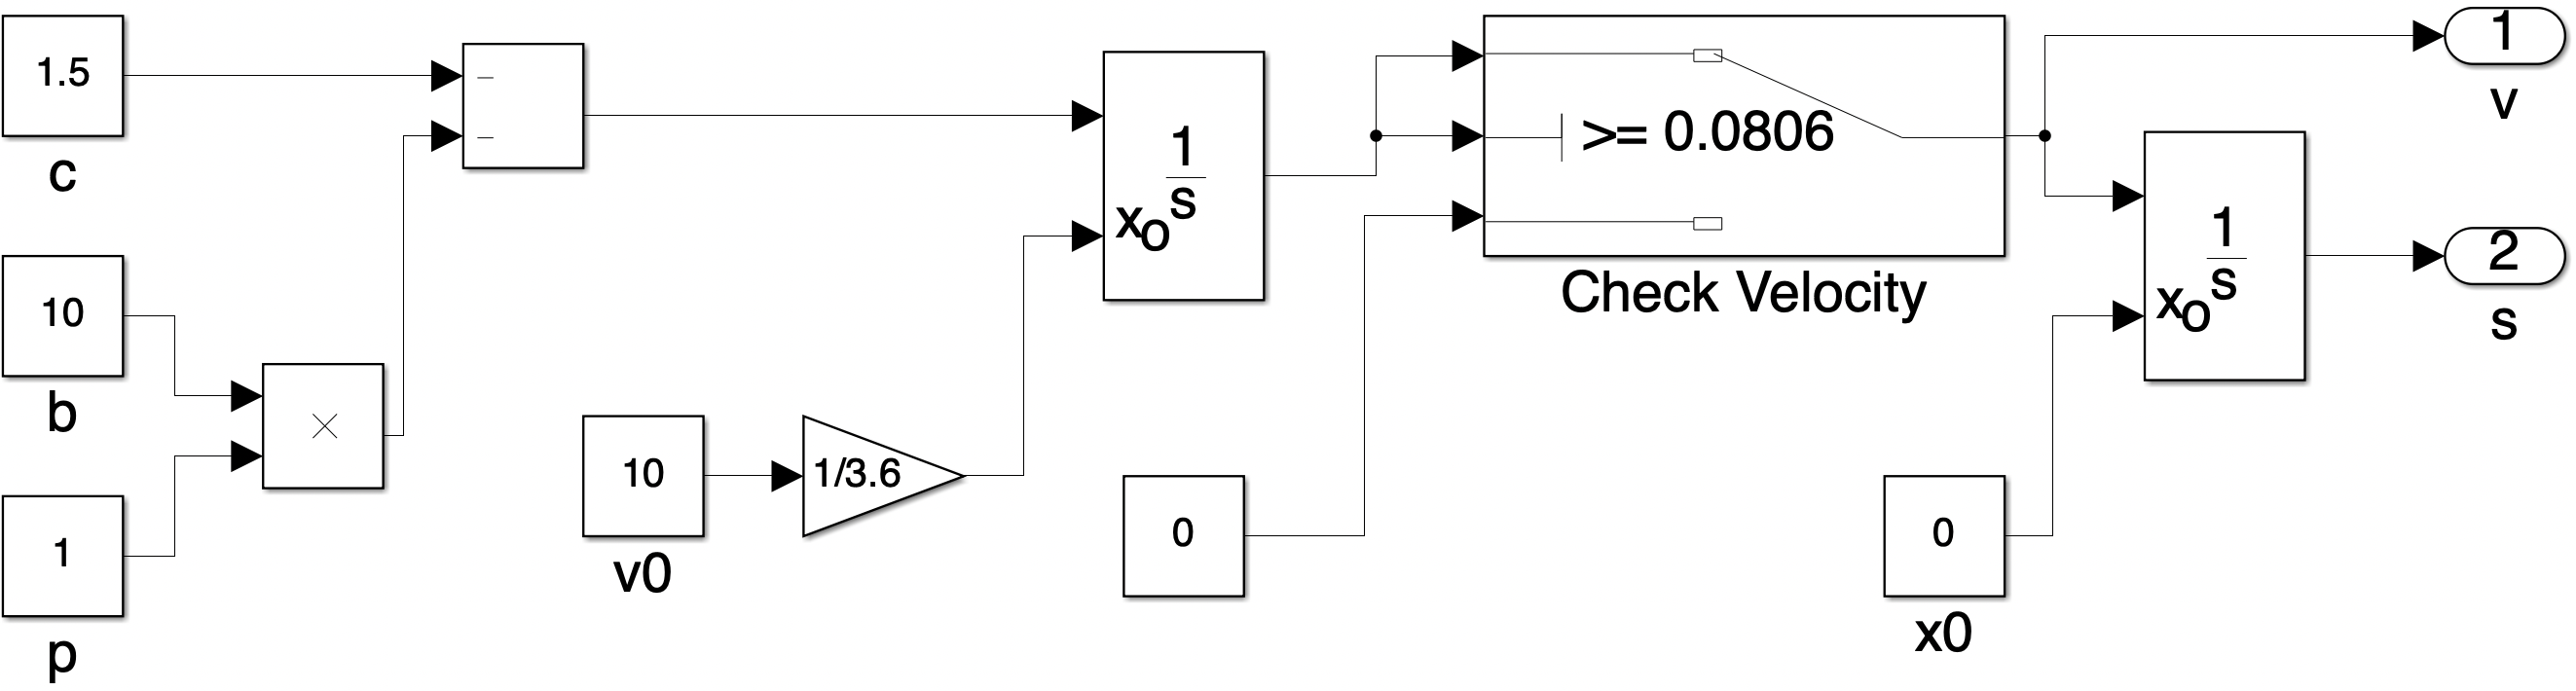
\includegraphics[width=1\textwidth]{images/D2_sim.png}
\caption{Simulink model of the differential equations}
\label{fig:D2_Sim}
\end{figure}

\section{Test scenario}\label{sec:D2_scenario}
The goal of this scenario is to check whether it is possible, with the given model, to realize a smooth stop with a stopping location < 2 m.
The idea is to demonstrate, that a full stop before 2 m can be realised with a reasonable brake pedal pressure and a reasonable deceleration.
If, for example a stop before 2 m could only be realised with 100 \% brake pressure, that would mean that a smooth stop can not be realised.\\
It is not necessary to implement a human-like smooth stop, but to show that this is possible.
Therefore the proposed test scenario is to run the model and find a reasonable small brake pressure where the car comes to a full stop with a location < 2 m.
This would show the feasibility of the task.
Creating a human-like brake profile where the brake parameter p can be adjusted over time is not an objective of this feasibility study, this will be covered at a later stage.\\
The execution of this scenario is automated using a Matlab script, which parametrizes the model and displays the outputs.
Listing \ref{lst:D2_matlab} shows the script that executes the simulation and stores the results.
The code to create the result plots has been excluded.
In lines one to eight the simulation is parametrized.
A stop time of 2 seconds is chosen because the car will come to a stop before.

todo solver begründen

The constant brake pressure is set to 5 \%.
This value results in a stop before the car traveled 2 meters of distance and is also reasonably small.

\begin{lstlisting}[language=Matlab,basicstyle=\scriptsize, caption= Execution of the feasibility test,label= lst:D2_matlab]
%% Parametrize Model
set_param('D2','StopTime','2');
%set solver
set_param('D2','Solver',['ode',sprintf('%d',8)]);
%set simulation step size
set_param('D2','FixedStep',sprintf('%f',0.01));
%set brake pressure parameter
set_param('D2/p','value',sprintf('%f',0.05));


%% Simulate and get output
res = sim('D2','SaveOutput','on','SaveState','on');
t = res.tout;
v = res.yout{1}.Values.Data;
s = res.yout{2}.Values.Data;
a = res.yout{3}.Values.Data;
%convert velocity to km/h
v = v*3.6;
\end{lstlisting}
\section{Results}\label{sec:D2_results}
The following figure \ref{fig:D2_Result} shows the simulation results with a constant brake pressure of 5\%. This results in a constant deceleration of -2 m/$s^2$. Setting the velocity to zero, when reaching the minimal velocity, has no impact on the computed acceleration. This is the reason, why the acceleration still remains the same, even though the car is not moving anymore.\\
The velocity linearly decreases from $v_0 = 10$ km/h to zero (except the decrease from minimal velocity to zero, which was expected).
The third subplot shows the covered distance of the car, which is clearly under the 2 m mark.
Therefore, with a constant brake pressure of 5 \% the car can be stopped before reaching 2 m travelled distance with an acceptable deceleration of 2 m/$s^2$. In the cruise control project we have discussed that an acceleration of less than 4 m/$s^2$ is not uncomfortable.\\
These simulation results demonstrate that it should be possible, with variation of the brake pressure over time, to realise a smooth stop with a human-like brake profile.

\begin{figure}[H]
\centering
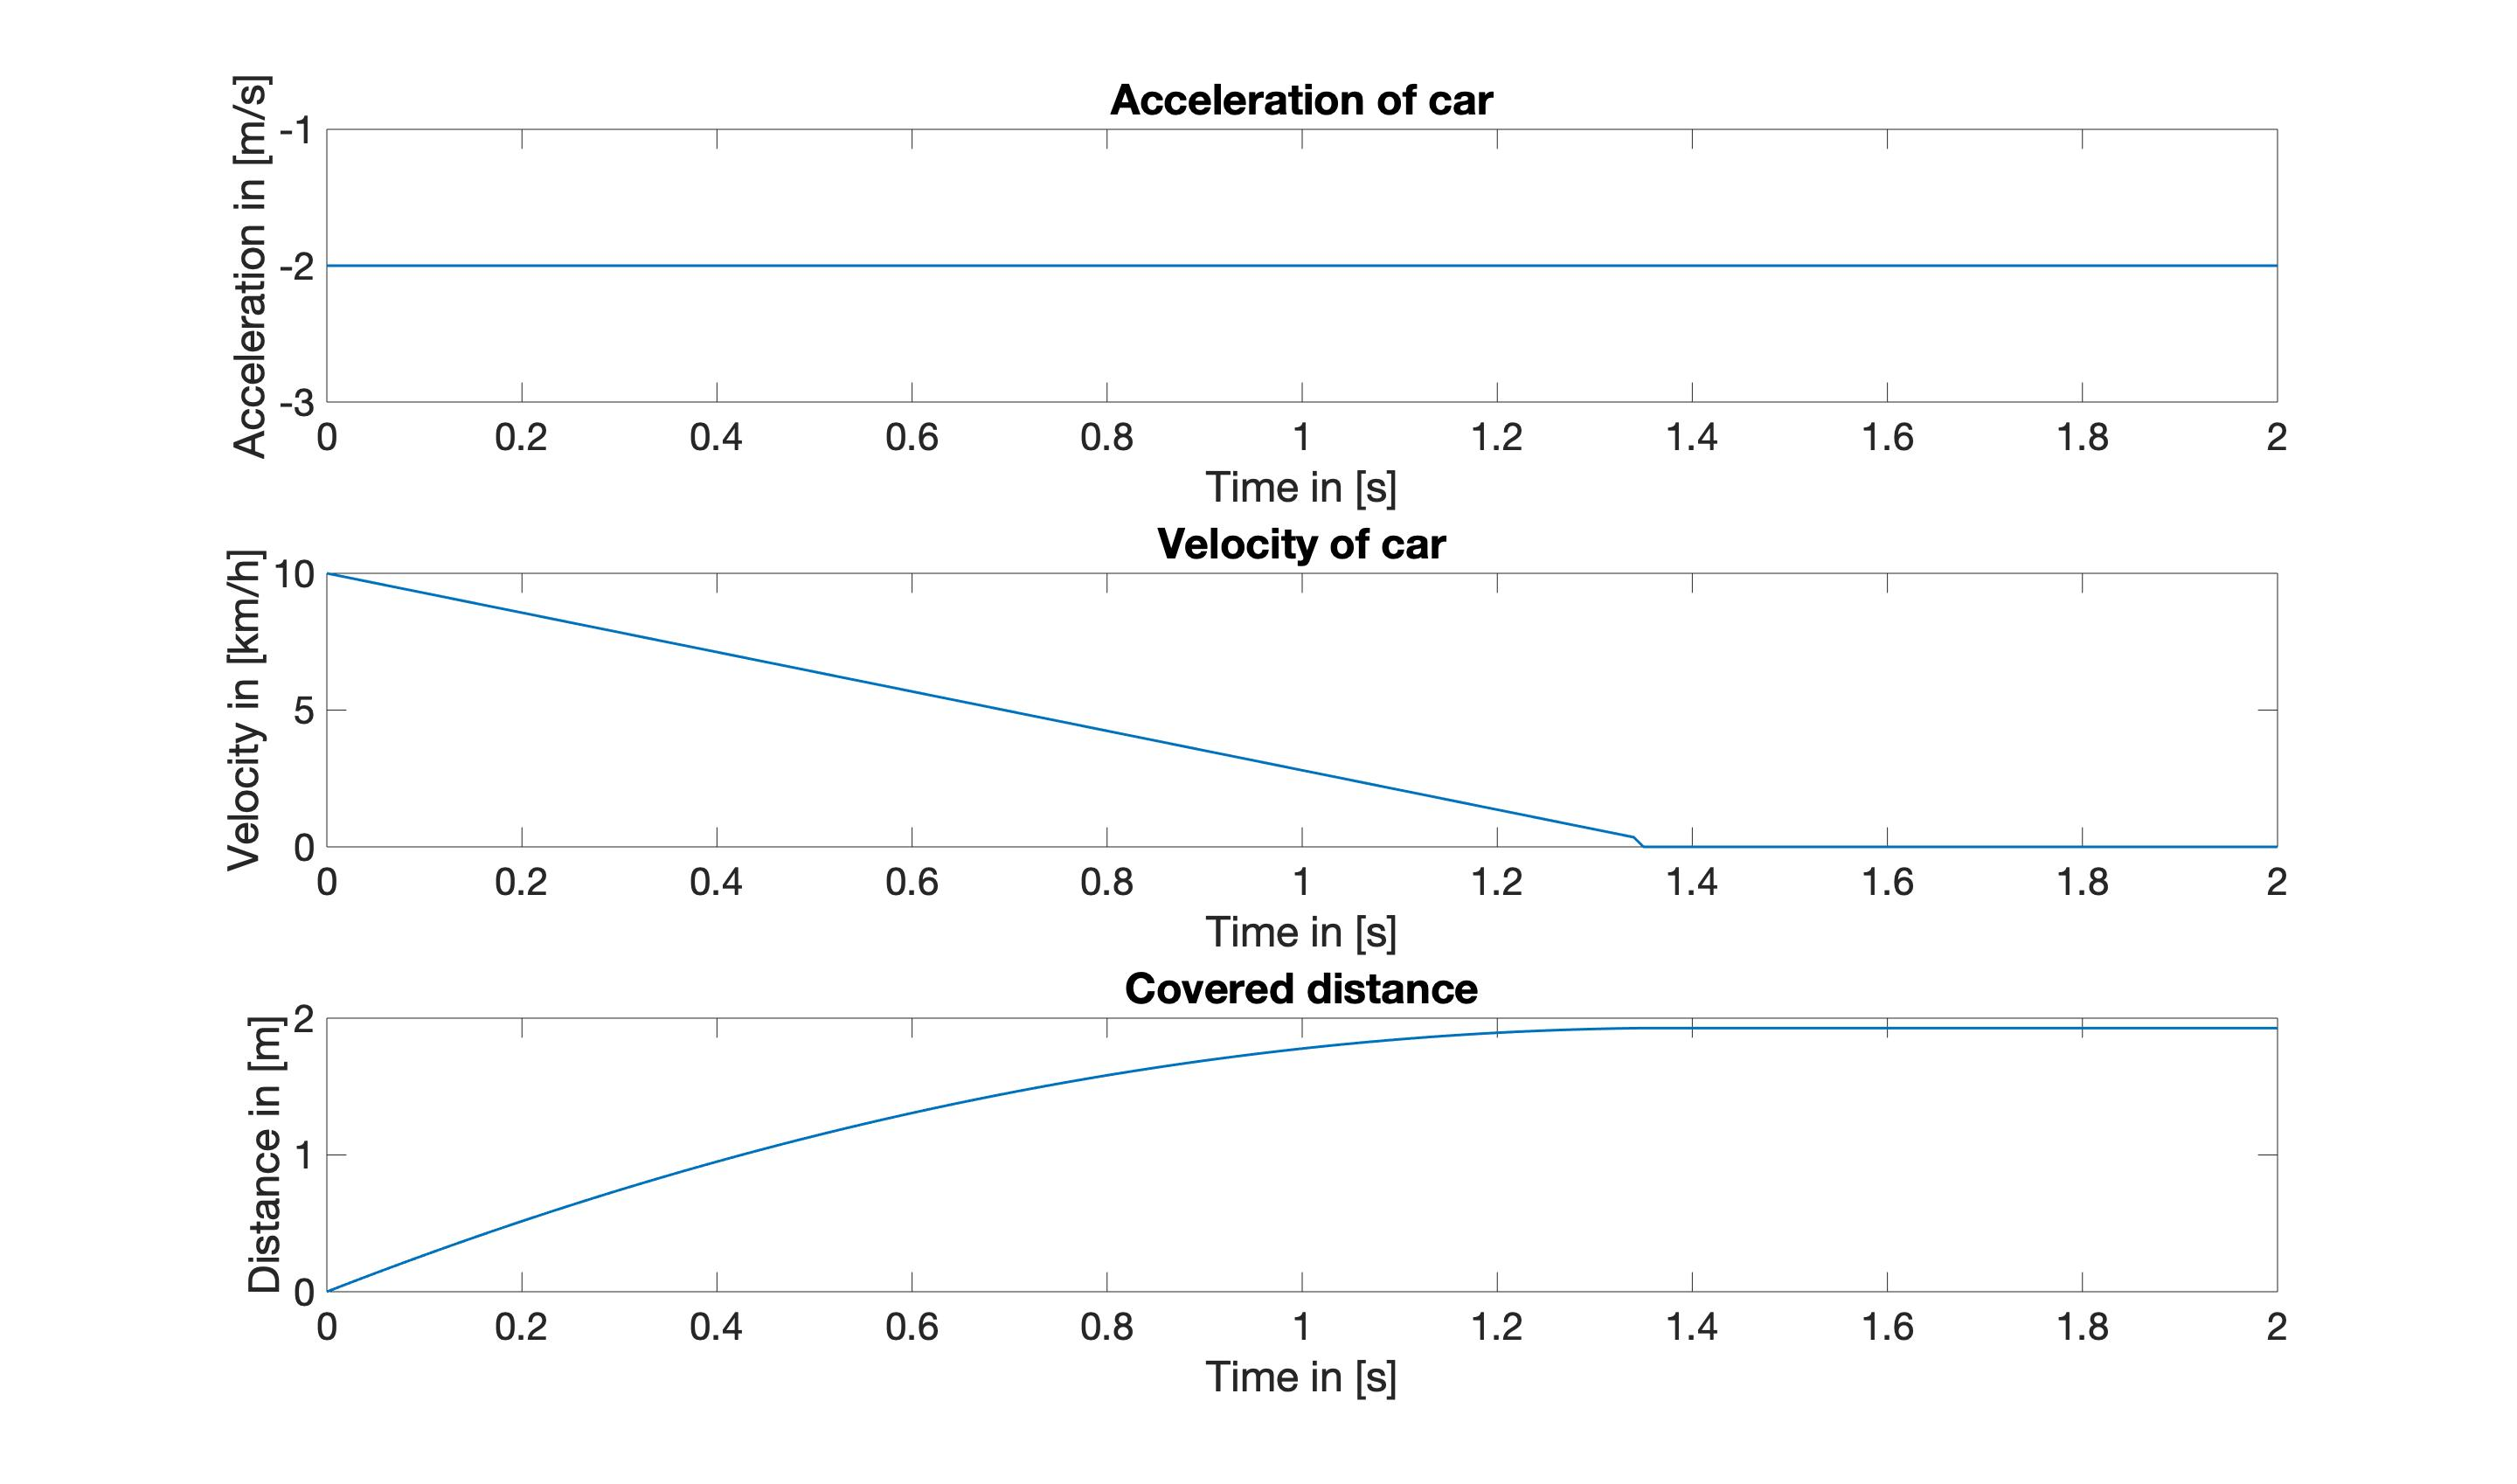
\includegraphics[width=1\textwidth]{images/D2_plot.jpg}
\caption{Simulation results of feasibility study}
\label{fig:D2_Result}
\end{figure}

\chapter{D3: Analysis of human velocity profile}\label{cha:D3}

In this section the provided human velocity profile is analysed in order to find a pattern that can be abstracted as a human-like brake profile.
This pattern will be used in the following sections and will be adapted to the braking function of the ParkAssist.
For the analysis Matlab functions are used, as demanded by requirement D3.
\section{Import the measurement data}
The human velocity profile contains a time dimension and the four wheel velocities.
The following listing shows how the measurement data is imported in Matlab.
A Matlab library function is used for the import of the textfile.
This results in a standard numeric matrix.

\begin{lstlisting}[language=Matlab,basicstyle=\scriptsize	,caption= Import measurement data in Matlab,label= lst:D3Import]
%import velocity data
velocity_data = importdata('MeasuredVelocities.txt');
\end{lstlisting}

\section{Data preparation}
Before analysing the data it is necessary to preprocess it. The aim is to make conclusions on a brake profile.
Since the brake pressure has a linear influence on the acceleration (model formula) it would be desirable to extract an acceleration curve from the human velocity profile, from which to make deductions on the brake profile.
For that, a car acceleration and in consequence car velocity is needed.
Therefore a car velocity has to be extracted from the four wheel velocities.\\

Listing \ref{lst:D3Preprocess} shows the matlab script, that does the preprocessing.
As a first step, the four wheel velocities are extracted from the measurement data and a mean velocity is calculated (lines 2 and 3) with the following equation:
\begin{equation}
	v_{car} = (v_{w1} +v_{w2} + v_{w3} +v_{w4})/4
\end{equation}
This mean velocity serves as an estimate for the car velocity.
It is only an estimate, because friction losses, other physical influences and cornering are not considered.
The mean velocity is converted to [m/s] for further calculations in line 4.
For analysing the braking behaviour the acceleration can be calculated by differentiating the mean velocity.
As can be seen in figure \ref{fig:D3_MovingAverage} in the upper subplot the calculated acceleration is noisy because of noise in the measured velocity.
Due to the noise it would be harder to analyse the braking behaviour. Therefore, we used a moving average filter to smoothen the data (line 8).
A moving average filter is calculating a mean value of neighbouring elements within a sliding window of a predefined size.
Applying a moving average filter results into a filtered graph that can bee seen in the lower subplot in figure \ref{fig:D3_MovingAverage}. 
However, applying a moving average filter distorts the acceleration values because the exact value is replaced by the average of the neighbouring elements. This reduces the difference between the values of neighbouring elements.
As a result the differentiation of the velocity results in an acceleration that is is in our case approximately 10 times smaller than the non-filtered results.
Although the values of the acceleration are smaller the relation of the acceleration is not changed.
Therefore the filtered data is not used to extract exact acceleration values, but to get an understanding of the acceleration curve during braking.\\

The movering average filter is applied in line 8. The sliding window has a size of 200 neighbouring elements. This means that for each data point the 200 neighbour points sorrounding that point are used in the filtered value computation. The factor 200 is chosen because it is big enough to reduce noise but is also small enough to maintain the general course of the graph. In line 11 and 12 the velocity is differentiated.
\begin{lstlisting}[language=Matlab,basicstyle=\scriptsize	,caption= Preprocessing measurement data,label= lst:D3Preprocess]
%compute mean velocity of all 4 wheels
velocity_per_wheel = velocity_data(:,2:5);
mean_velocity = mean(velocity_per_wheel,2);
mean_velocity = mean_velocity/3.6;      %convert velocity from km/h to m/s
raw_mean_velocity = mean_velocity;      %for demonstration purposes

%apply moving average filter to smoothen the data
mean_velocity = movmean(mean_velocity, 200); 

%differentiate velocity to get acceleration
acceleration = diff(mean_velocity);
raw_acceleration = diff(raw_mean_velocity);     %for demonstration purposes
\end{lstlisting}

Figure \ref{fig:D3_MovingAverage} shows the impact of the moving average filter on the car velocity.
The course of the graph still the same, even though the absolute values are smaller that the unfiltered acceleration because of the before mentioned reasons.
\begin{figure}[H]
\centering
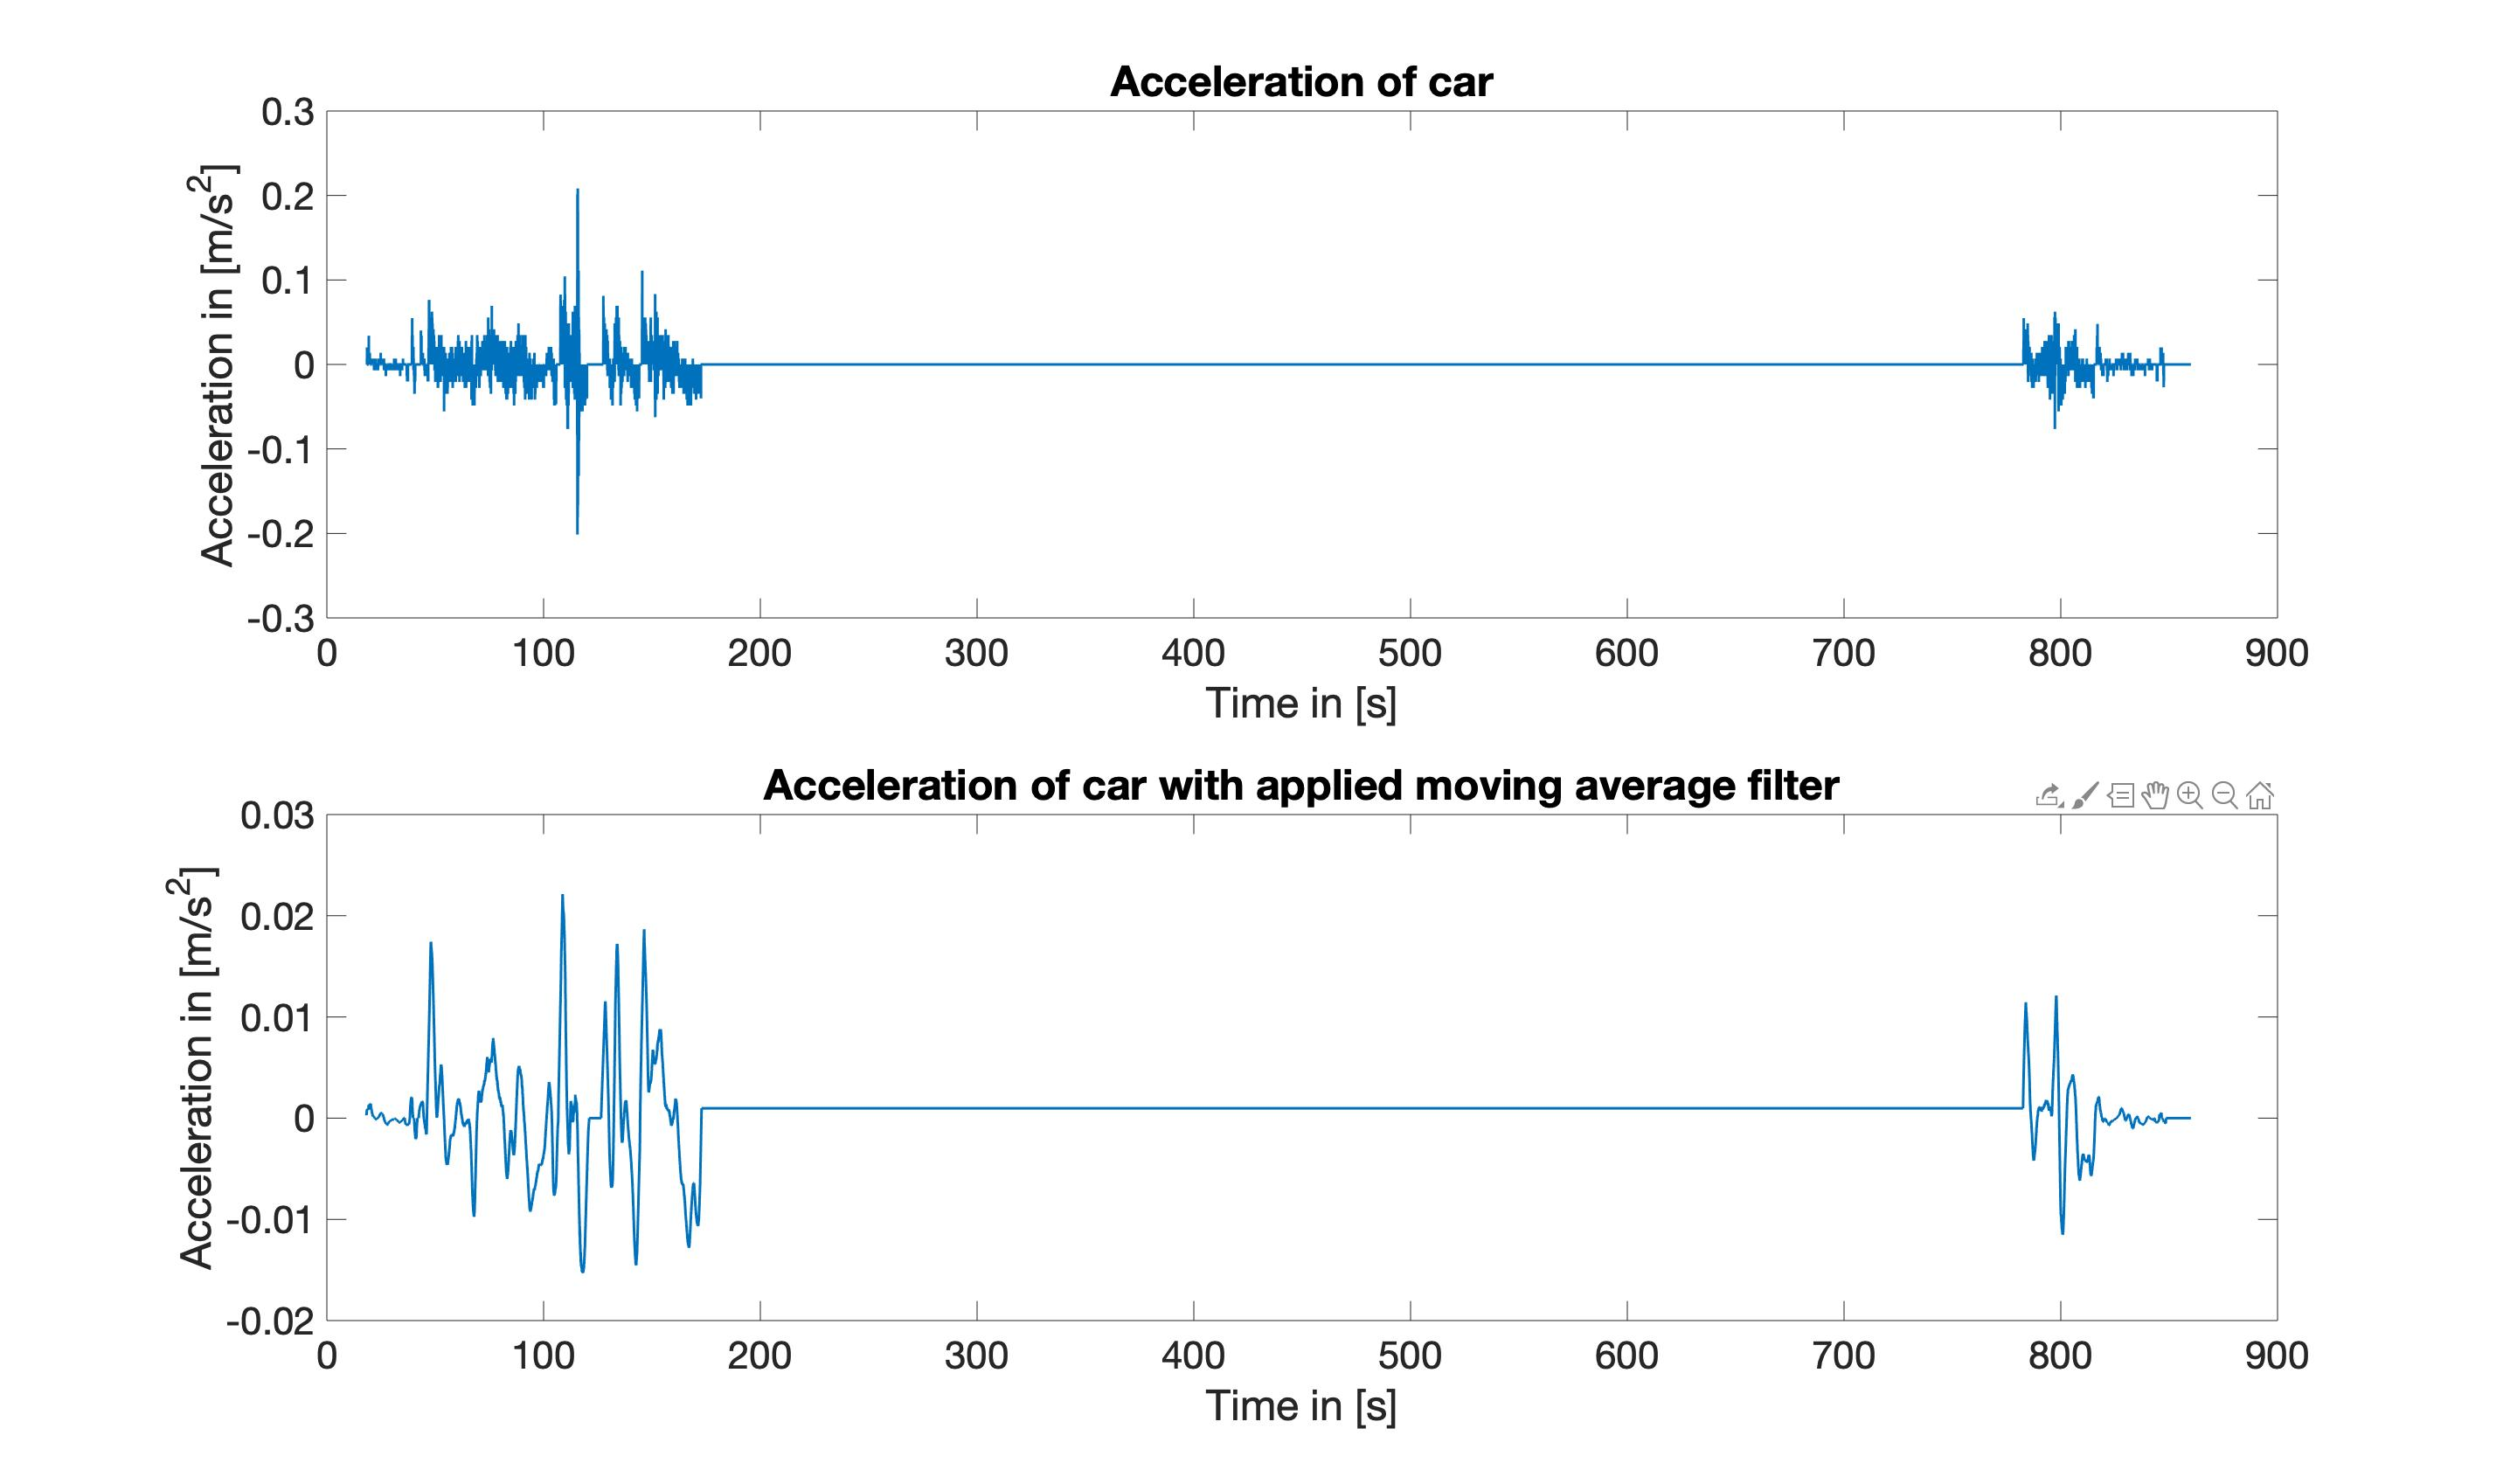
\includegraphics[width=1\textwidth]{images/D3_moving_average.jpg}
\caption{Impact of applying a moving average filter on the cars acceleration}
\label{fig:D3_MovingAverage}
\end{figure}

Figure \ref{fig:D3_Fig_Overview} shows the smoothed extracted mean velocity of the car as well as the corresponding acceleration of the car over time.

\begin{figure}[H]
\centering
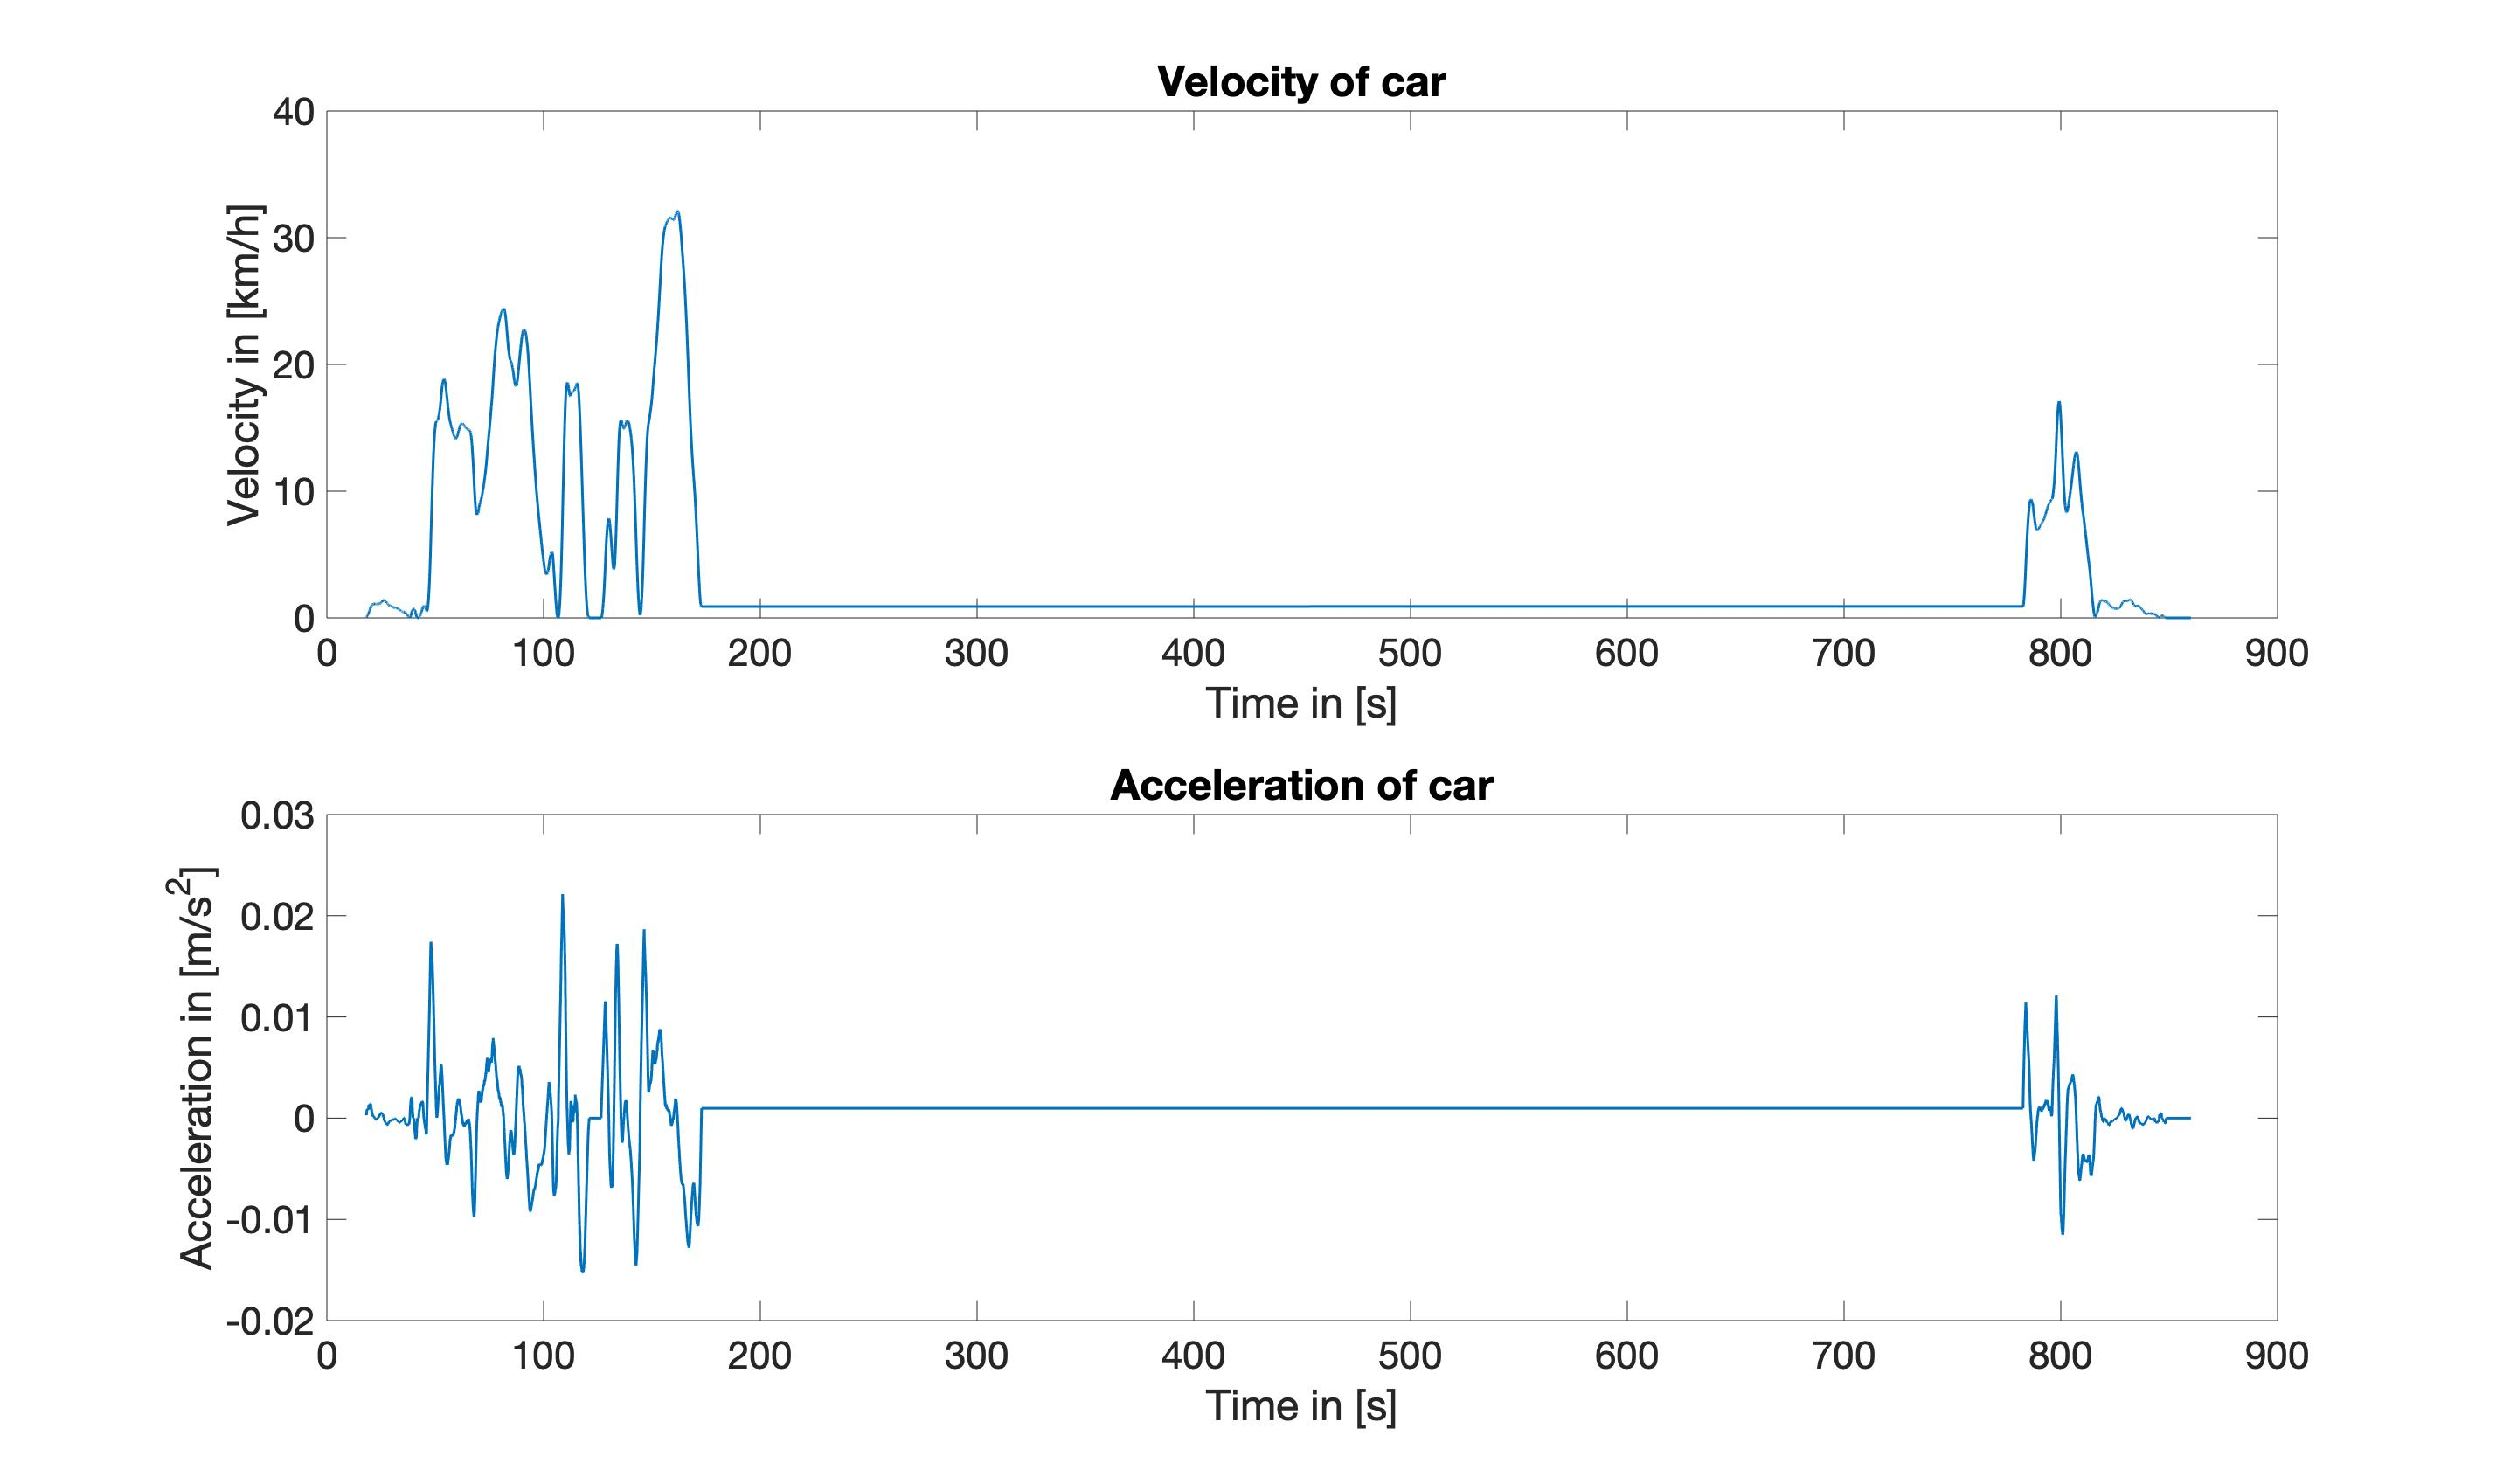
\includegraphics[width=1\textwidth]{images/D3_Fig_Overview.jpg}
\caption{Extracted human velocity profile}
\label{fig:D3_Fig_Overview}
\end{figure}


\section{Extracting negative acceleration}
As the goal is to analyse the braking behaviour only the negative acceleration is relevant and is thus being extracted from the overall acceleration (line 5). Also, all velocities that are based on a positive acceleration are not considered anymore (line 6). We decided to set those values to \ac{NaN} because this way we are still able to plot the velocity and the acceleration over time without cut-outs. The result can be seen in plot REF. todo create plot

\begin{lstlisting}[language=Matlab,basicstyle=\scriptsize	,caption= Extracting negative acceleration,label= lst:D3Extract]
%search for negative acceleration and set positive acceleration to NaN
%set all velocities that have a positive acceleration to NaN
neg_acceleration = acceleration;
decreasing_velocity = mean_velocity;
neg_acceleration(neg_acceleration>0) = nan;
decreasing_velocity(isnan(neg_acceleration)) = nan;
\end{lstlisting}


\section{Separating breaking sequences}
For improved visualisation the individual breaking sequences that can be seen in plot \ref{fig:D3_IndividualBraking} are stored separately.
One breaking sequence consists of multiple consequent velocities.
This means that the breaking sequences can be separated by searching for a gap in the velocities.
Therefore, the indices of all velocities that are set not \ac{NaN} are extracted (line 2) and differentiated (line 3).
Considered the differentiation, every differentiation that is greater than 1 marks a gap between velocities because indices of one braking sequence are consequent (differentiation equals 1).
Furthermore, small breaking sequences are not considered because they are most likely not relevant for recognizing a breaking pattern (line 13).
Two individual breaking sequences can be seen in plot \ref{fig:D3_IndividualBraking1} and plot \ref{fig:D3_IndividualBraking2}.

\begin{lstlisting}[language=Matlab,basicstyle=\scriptsize	,caption= Separating breaking sequences,label= lst:D3Seperat]
%find individual breaking sequences
notNaN_velocity = find(~isnan(decreasing_velocity));   % find index of every velocity that is not NaN -> one breaking sequence has consequent time steps -> one breaking sequence has consequent indices
diff_notNaN_velocity = diff(notNaN_velocity);          % differentiate indices -> if indices are not consequent (unequal 1), a new breaking sequence has begun
n = 1;                                                 % set start values
start = 1;

%seperate breaking sequences with previous findings
for i=1:length(diff_notNaN_velocity)
    %for every index check if indices are consequent -> equals 1
    if diff_notNaN_velocity(i) > 1
        %if not check if a breaking sequence consists of min 500 time
        %steps, this way small breaking sequences are sorted out
        if (i-start) > 500
            %add breaking sequence to section
            %i is end of sequence
            section{n} = notNaN_velocity(start:i);
            %start for new sequence is end of old sequence + 1
            start = i+1;
            %increment n
            n = n+1;
        else
            %if breaking sequence is to small, set start for new sequence
            %to end of old sequence + 1 anyway
            start = i+1;
        end
    end
end
\end{lstlisting}

\begin{figure}[H]
\centering
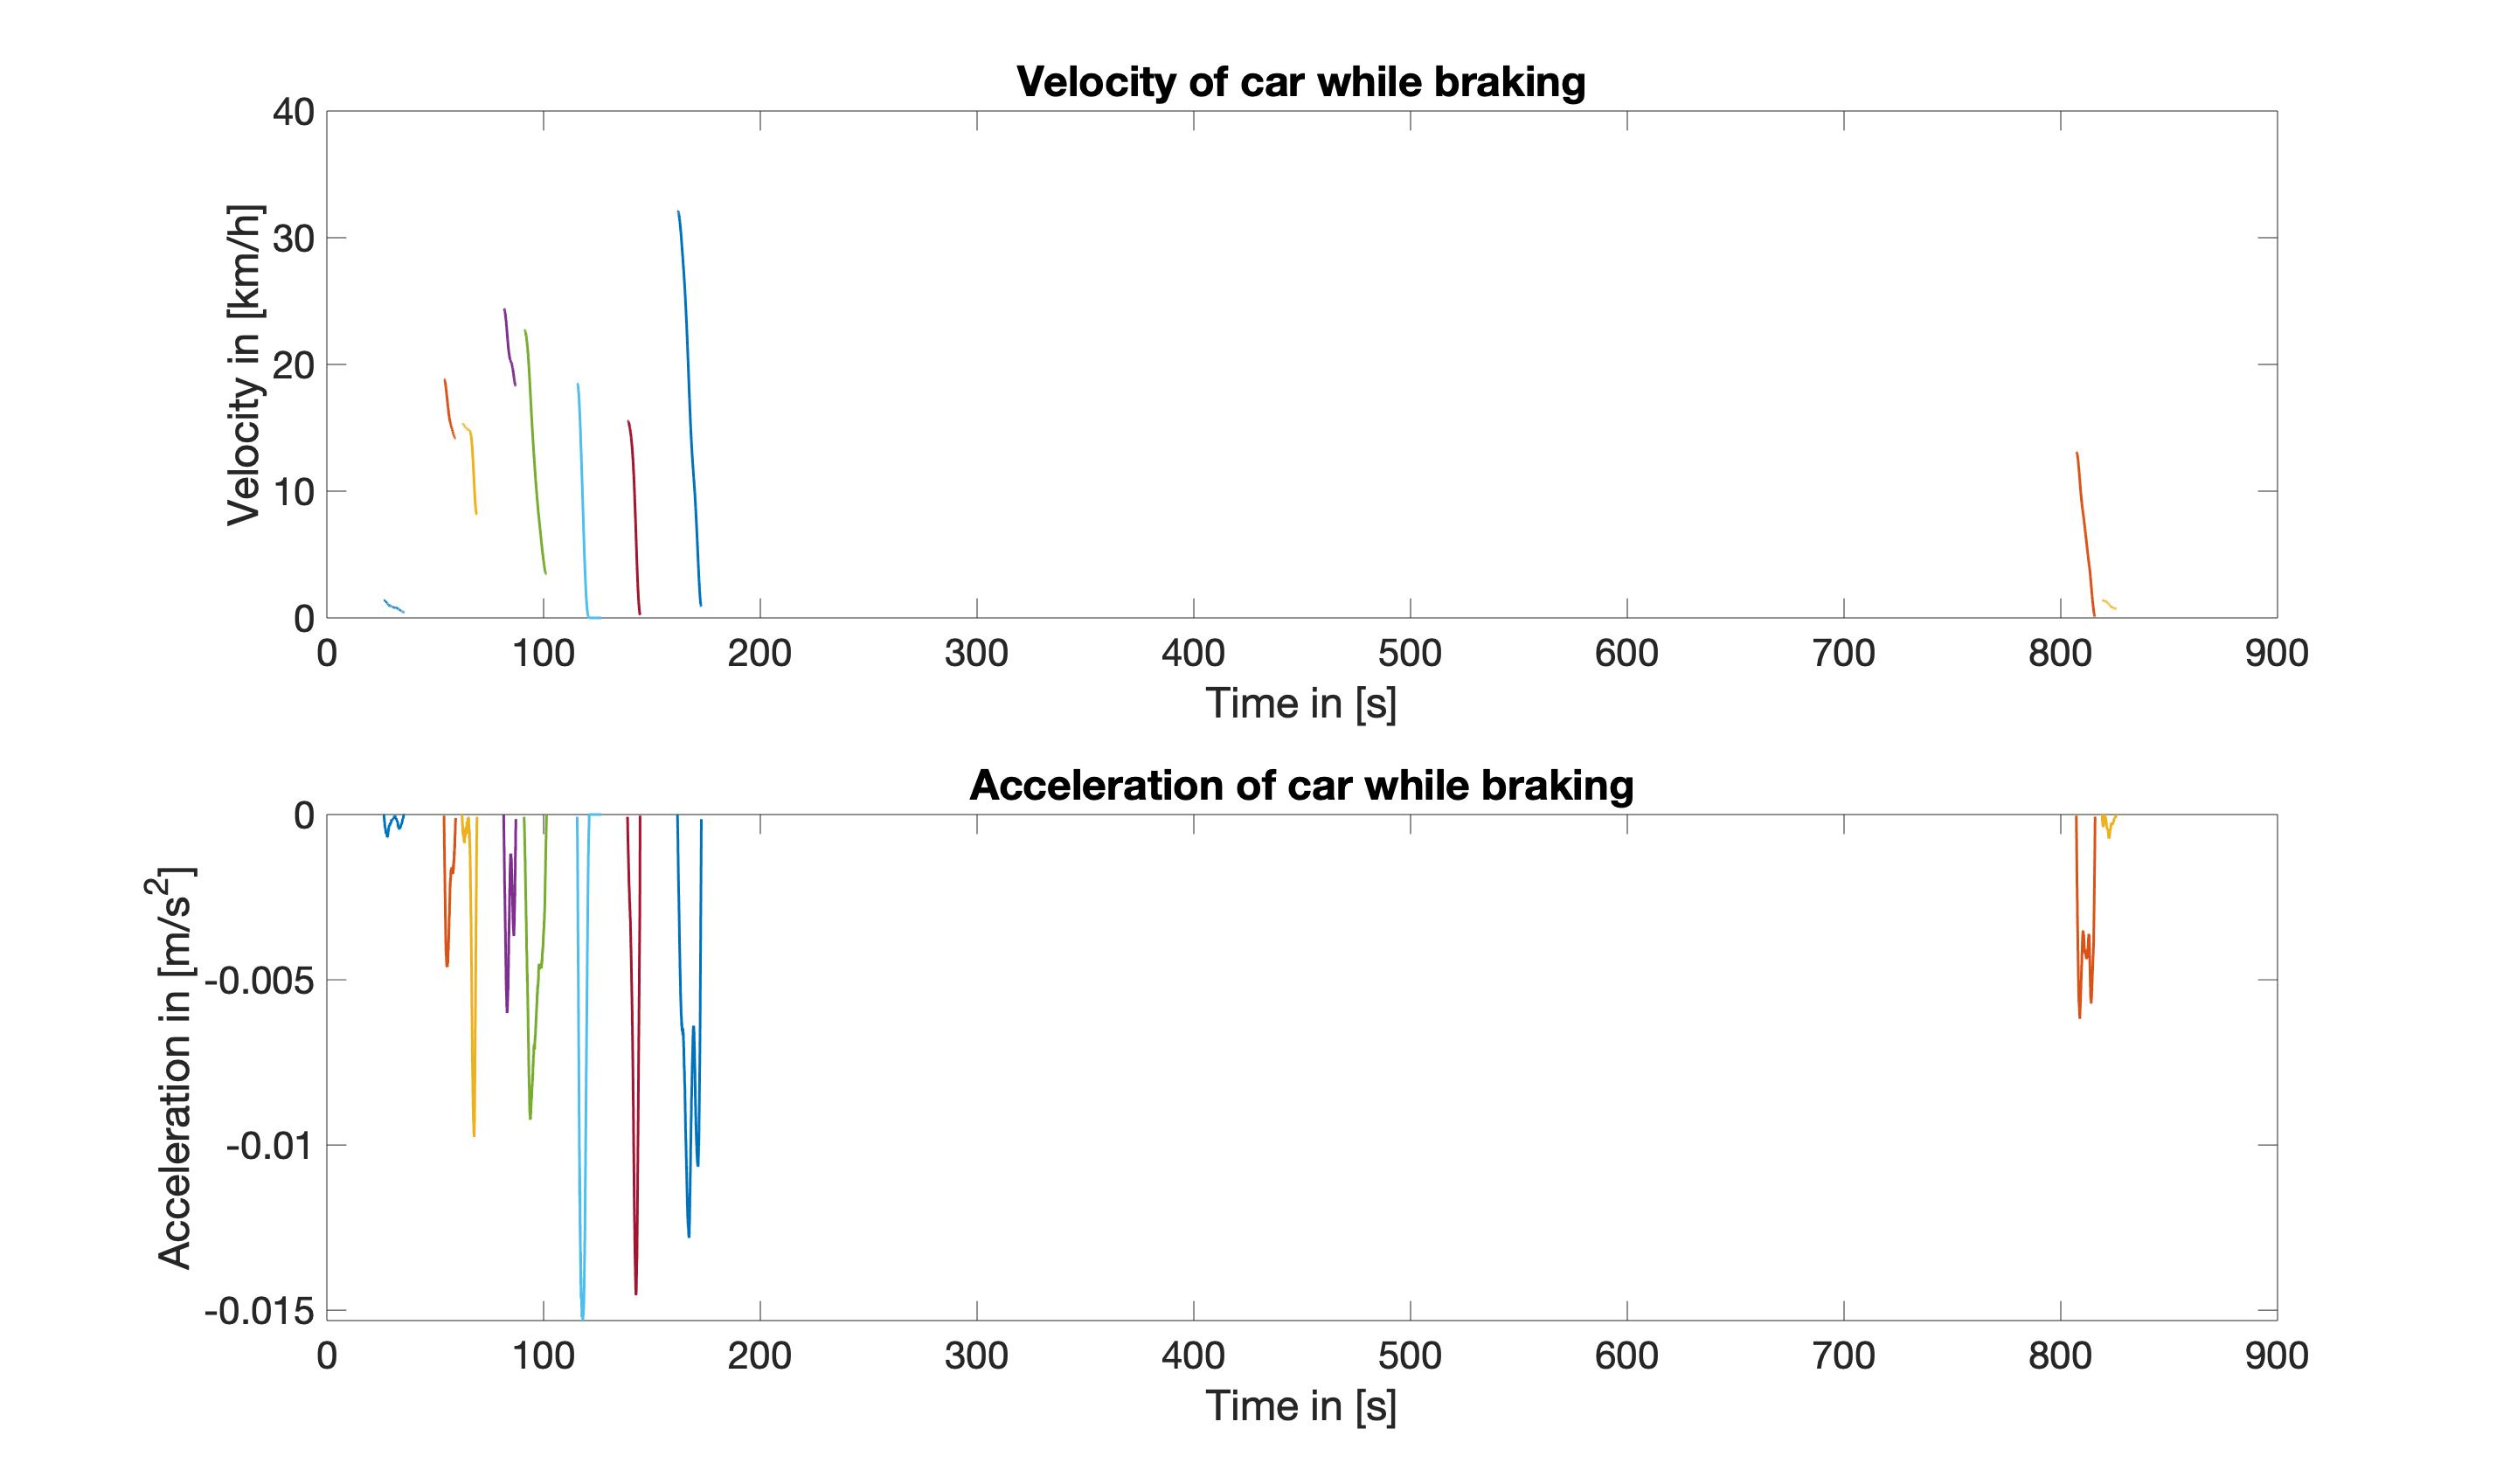
\includegraphics[width=1\textwidth]{images/D3_individual_braking.jpg}
\caption{Human velocity profile extracted individual braking manoeuvres}
\label{fig:D3_IndividualBraking}
\end{figure}

\begin{figure}[H]
\centering
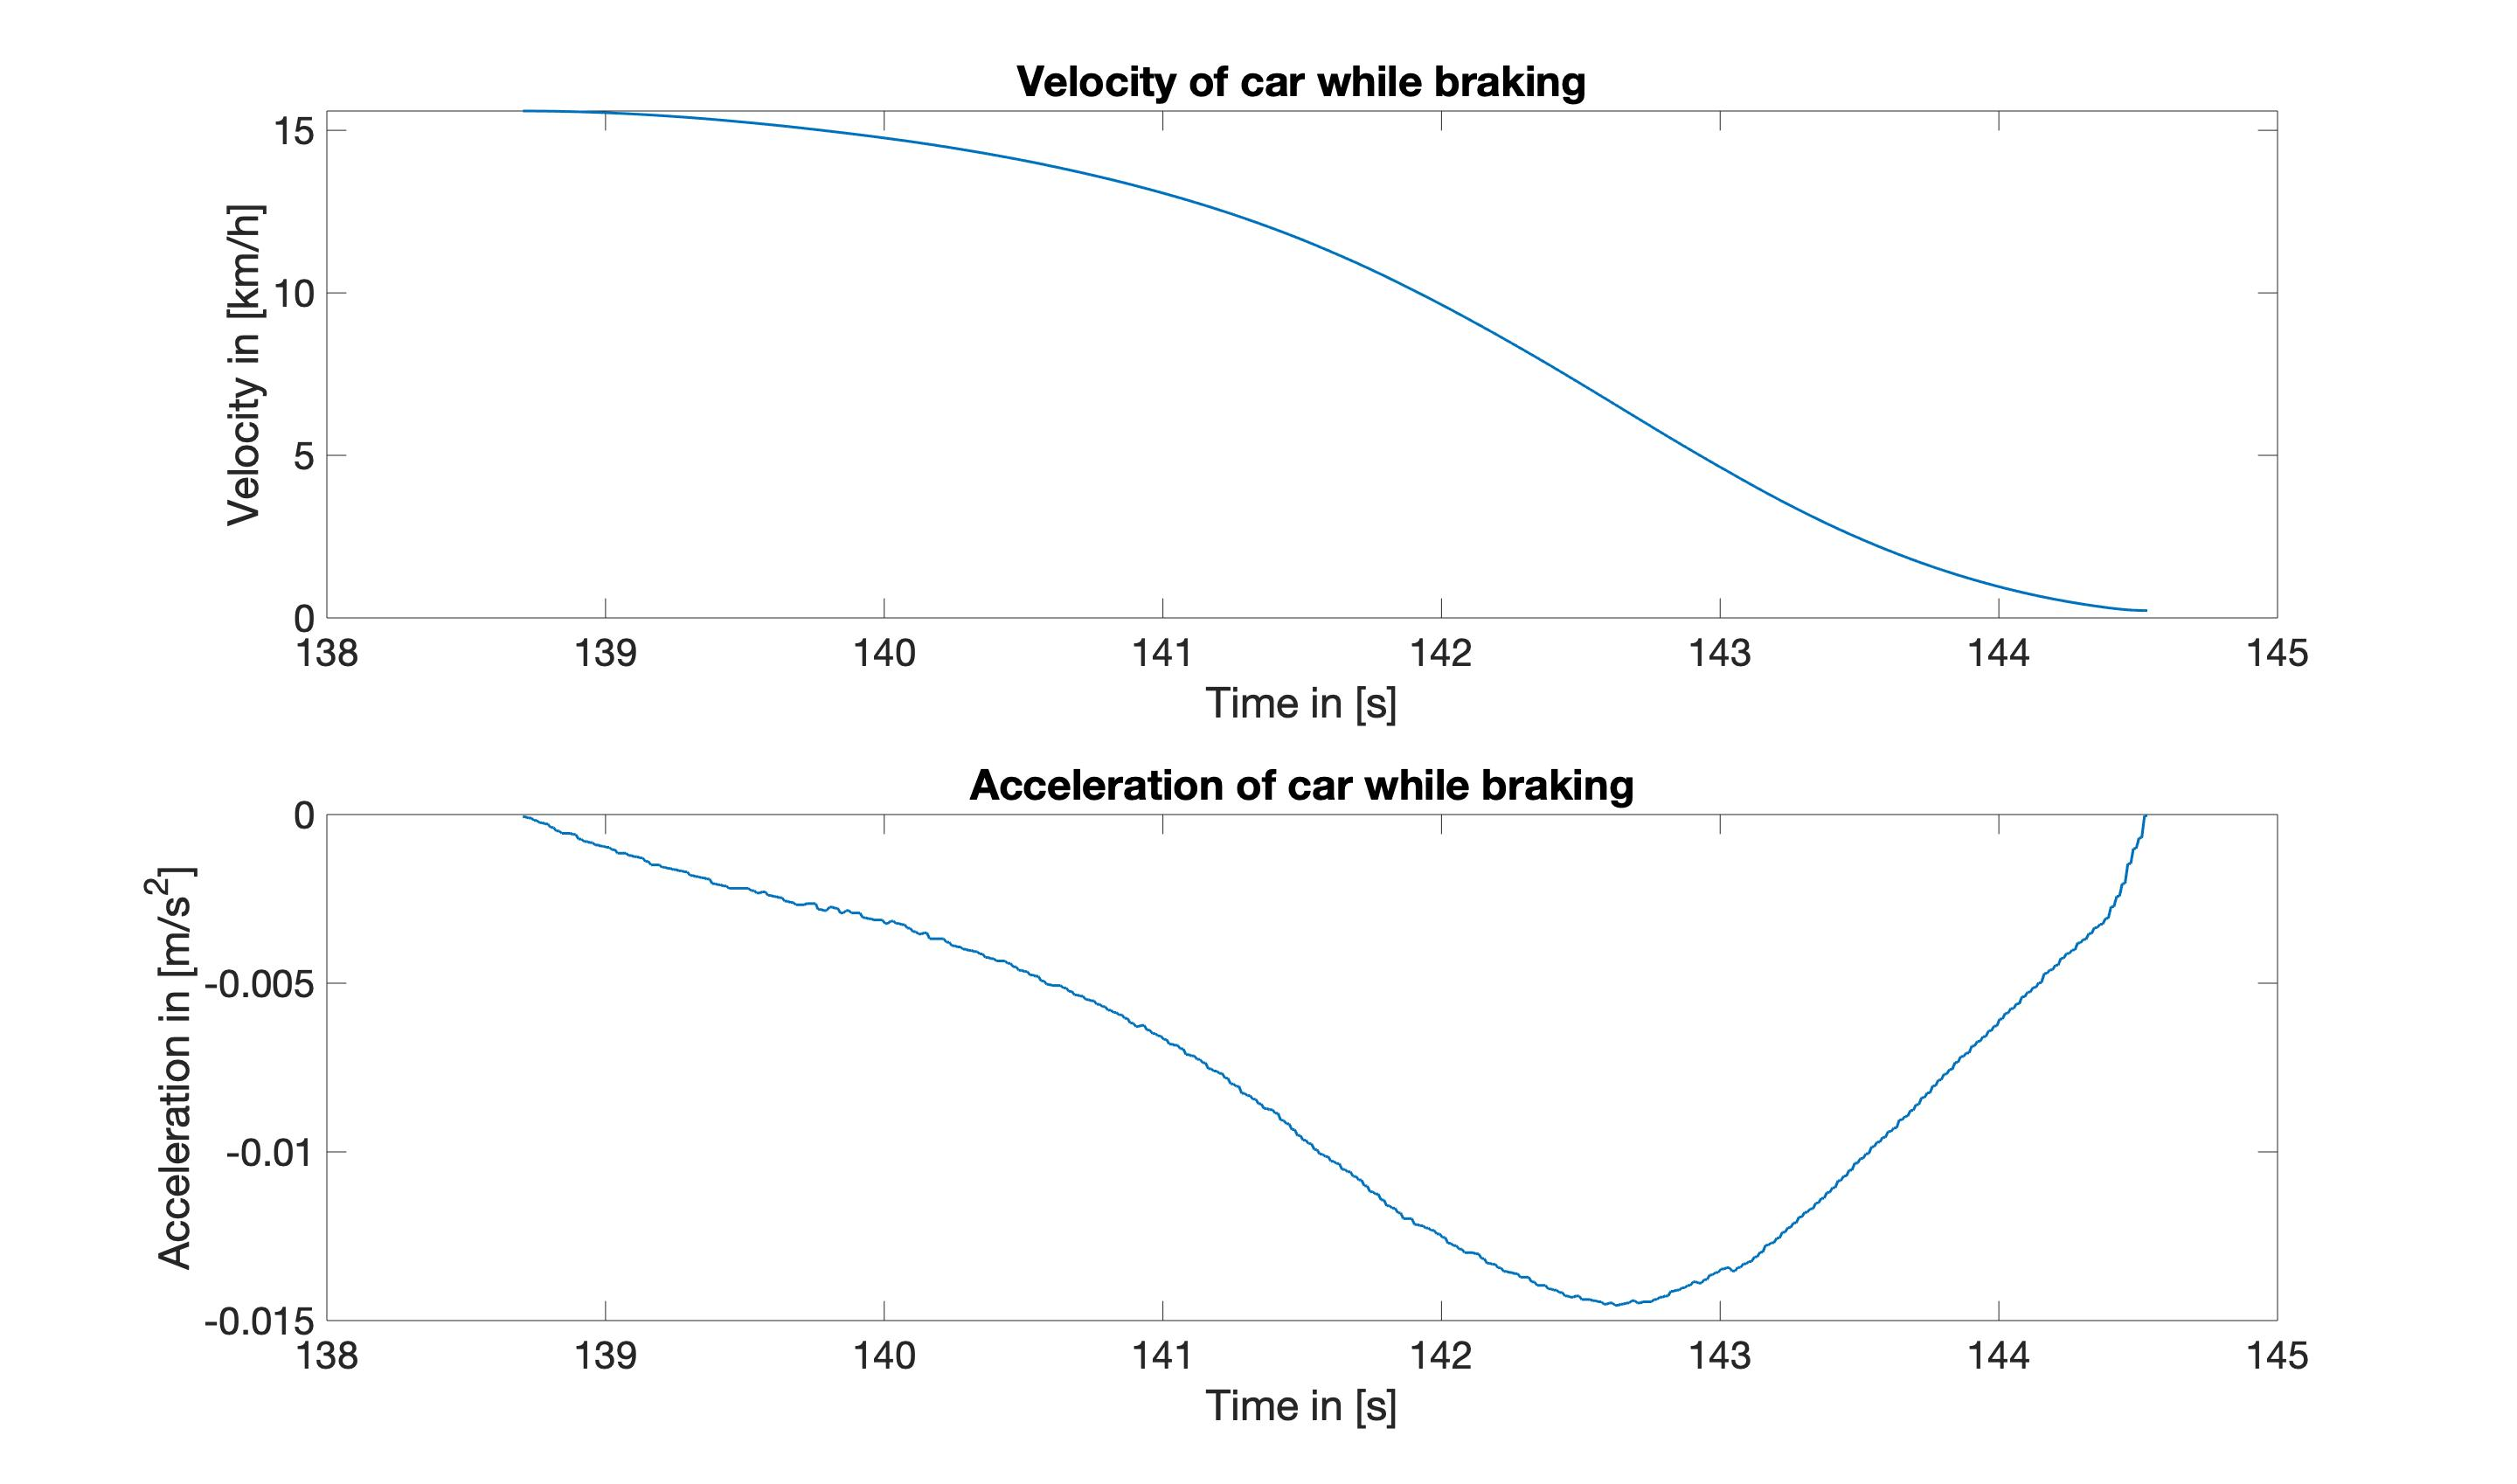
\includegraphics[width=1\textwidth]{images/D3_example1.jpg}
\caption{Human velocity profile extracted braking manoeuvre 1}
\label{fig:D3_IndividualBraking1}
\end{figure}

\begin{figure}[H]
\centering
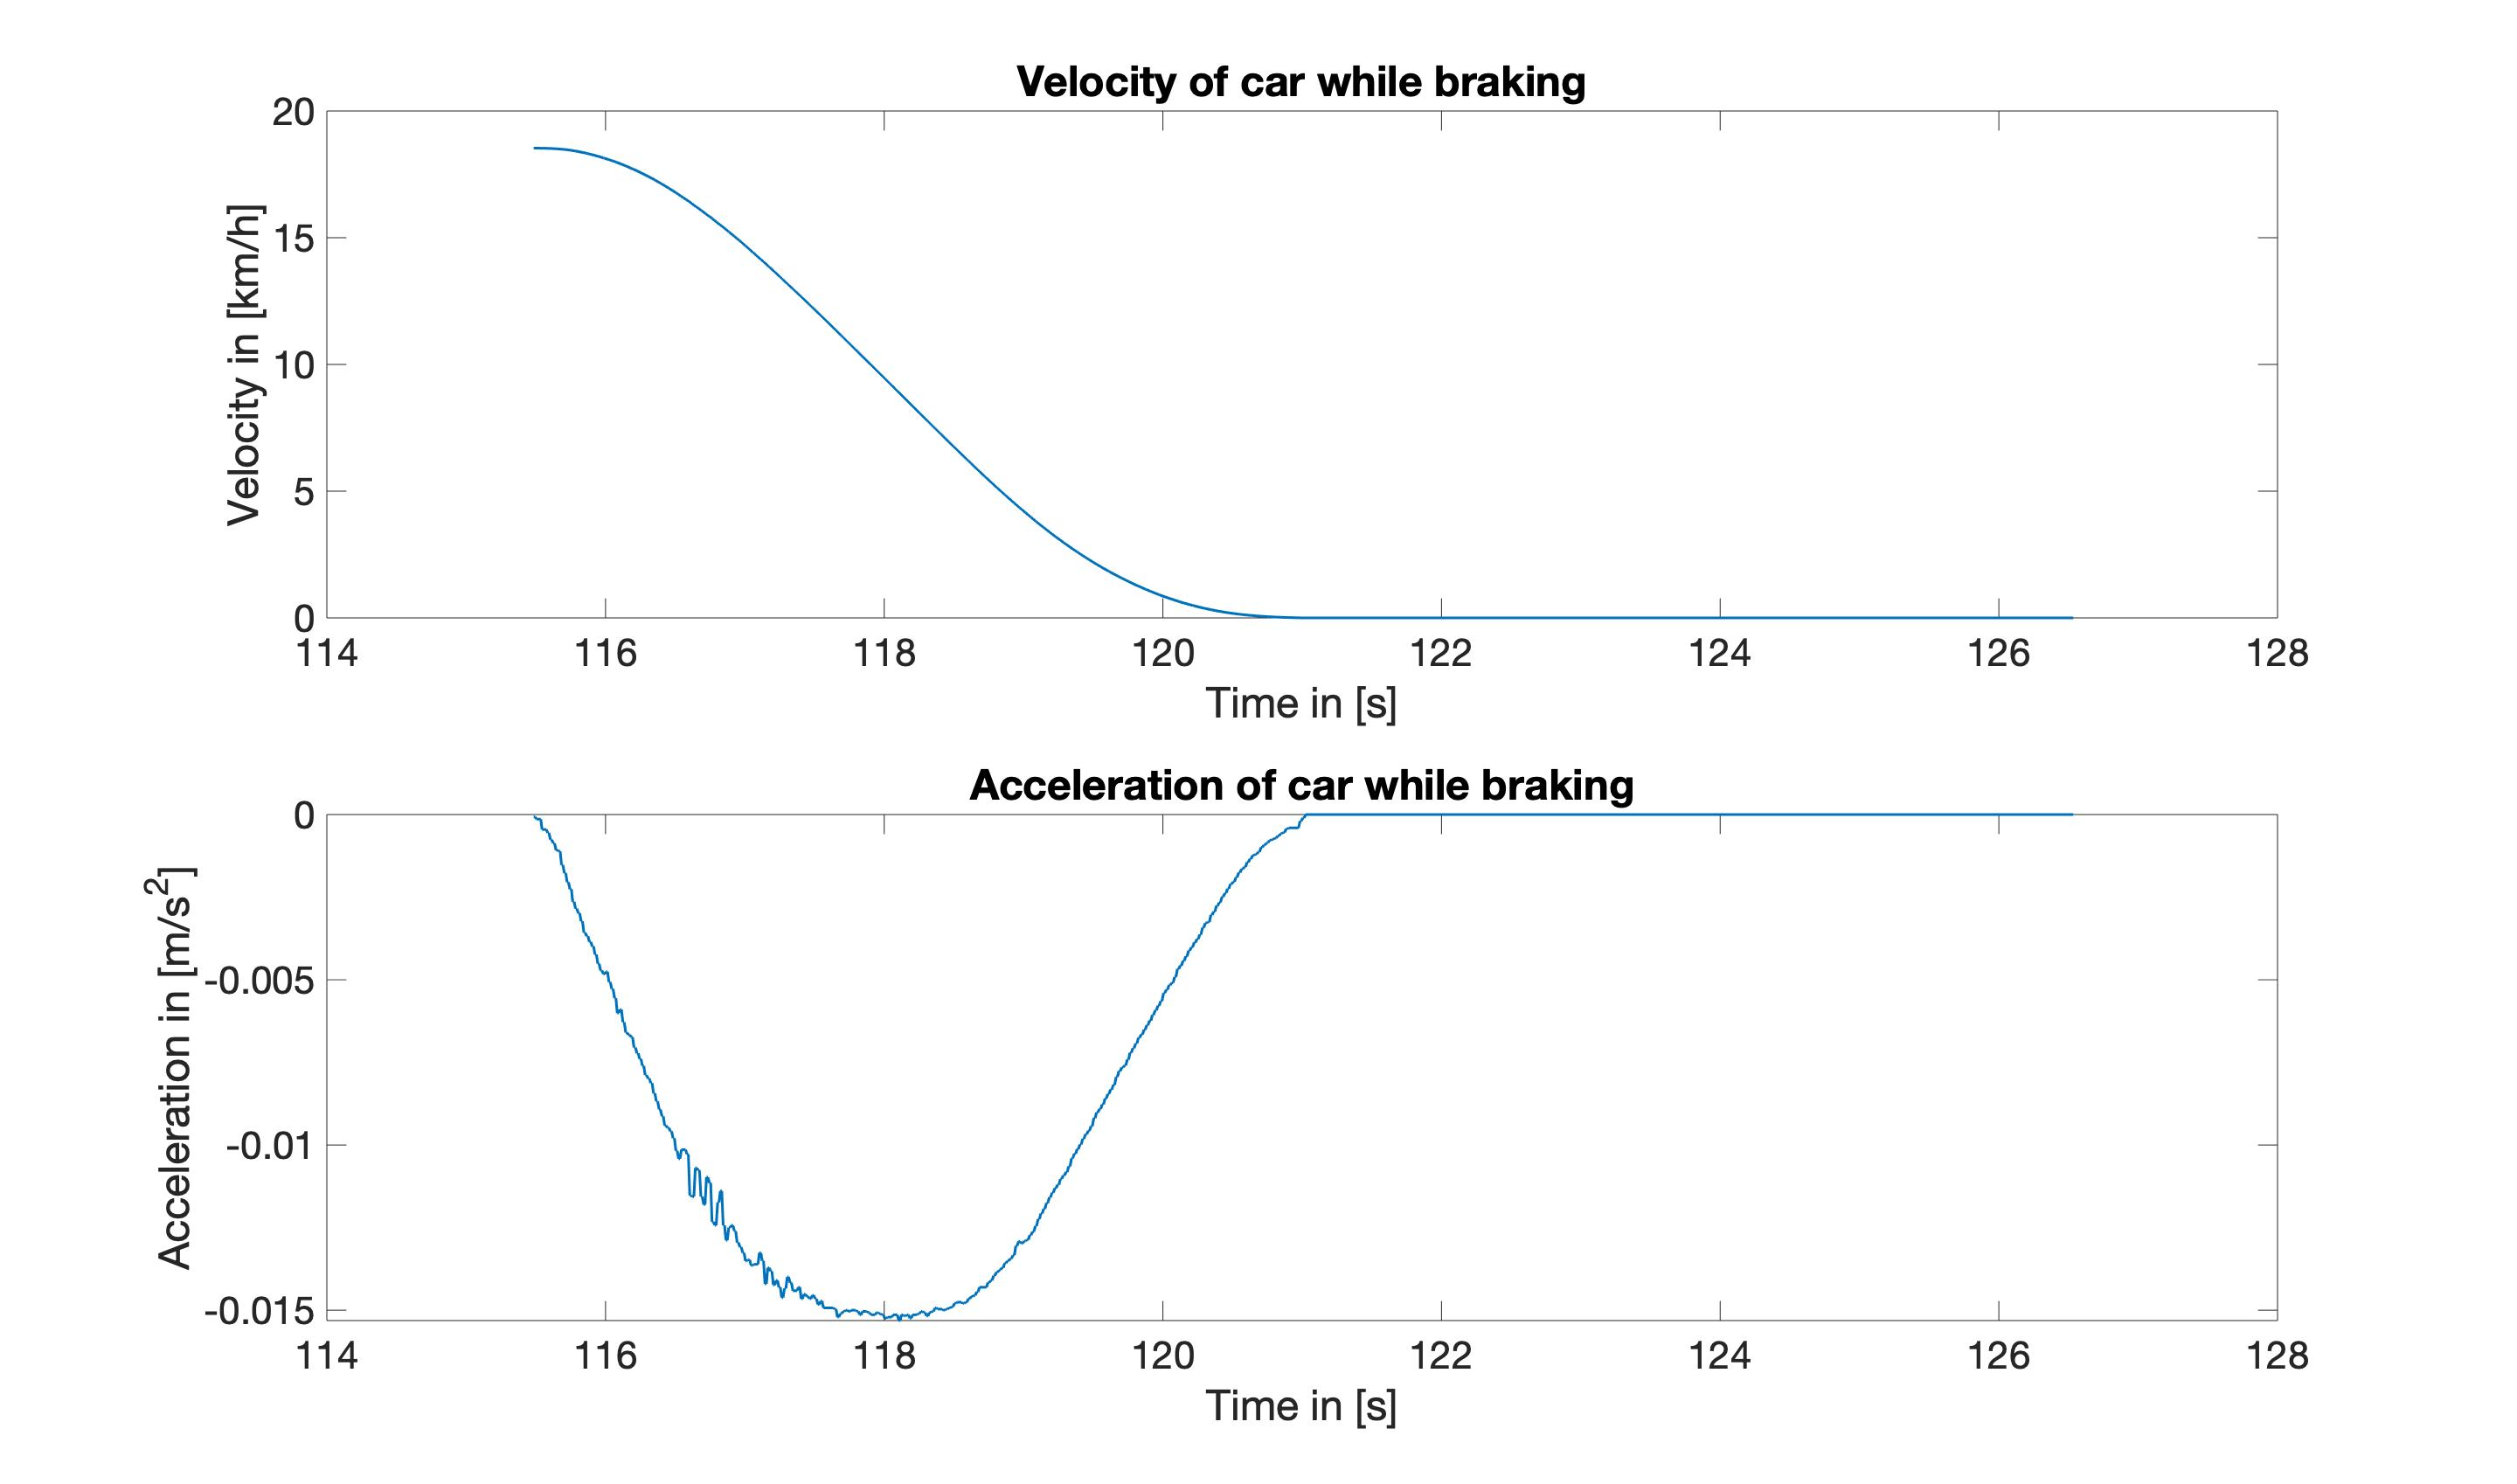
\includegraphics[width=1\textwidth]{images/D3_example2.jpg}
\caption{Human velocity profile extracted braking manoeuvre 2}
\label{fig:D3_IndividualBraking2}
\end{figure}

\section{Result}
Considering Figures REF, REF and REF, it can be seen that the acceleration is approximately in the shape of a parable with the minimal turning point at XX. For further implementation of the ParkAssist, we will start the breaking process with an acceleration and increase it until we reach approximately REF and will then decrease it.

%entschieden Durchschnitt der vier Radgeschwindigkeiten zu nehmen (vllt. vor nachteile)
%und so auf die Geschwindigkeit des Autos näherungsweise zu bestimmen
%
%todo hier plot von gesamtgeschwindigkeit
%
%idee: verzögerungsphasen extrahieren um so auf "menschliche" negative beschleunigung zu schließen
%problem: verrauschte messdaten -> dadurch ständiger wehcsel positive negative beschleunigung
%
%lösung: moving average filter zum glätten der messwerte
%dann extrahieren der negativen beschleunigungen

\chapter{D4*: Consideration of uneven parking spaces}\label{cha:D4}
-diagram

-forces need to be considered (hangabtriebskraft)

-negative slope would increase stopping time and position

-positive slope would make stopping time shorter

-negative slope critical since collision could occur

-therefore brake power would have to be increased or decreased

-physical borders need to be considered

-also when the car is stopped it should not start to roll forwards or backwards.
On a plain surface, the brake can be released, after the car is stopped.
A brake assist on a positive or negative slope would need to keep holding the brake or engaging the handbrake.

In the model without a minimum velocity, the velocity would become negative on braking instead of the car coming to a full stop.

\chapter{D5: Discussion of inaccuracies in velocity measurement}\label{cha:D5}
-inaccuracy of velocity +- 0.1 km/h
-also minimal velocity is 0.29 km/h which is not realistic, because velocity does not drop from 0.29 km/h to zero
-in human velocity profile 4 tire velocities recorded
-mean used to compute car velocity
-because of inaccuracy in velocity computed acceleration also has inaccuracy
-car driving around corner
validate findings by numbers from simulation

\chapter{D6: Implementation of pulse signal in Simulink}\label{cha:D6}

In D6 a pulsing information signal is described. This chapter documents the implementation of that signal.
Both signals are needed for the frequency computation.
The pulsing signal should only be present if the nonzero velocity of the car is $\leq$ 1 m/s and the position of the car is between 1 and 2 meters. From a frequency of 1 Hz at 1 meter it should rise up to 9 Hz at 1.9 meters. If the traveled distance is greater than 1.9 meters, the signal should become continuous.\\
This requirement can be divided into two separate compontents with separate responsibilities.\\
In the first component it is determined in which state the signal is (off, pulsing, continuous) and in the case of a pulsing signal the frequency of that pulse is computed.\\
The second component is responsible for outputting the pulse signal corresponing to the output of the first component.\\
The components are implemented using simulink subsystems which enables re-usability, encapsulation and also creates a better overview when looking at the main simulink model.\\
\section{Computation of pulse signal frequency}\label{sec:D6Frequency}
Figure \ref{fig:D6_Frequency_Computation} shows the simulink subsystem for the computation of the frequency of the pulse signal.
The inputs are the velocity and position of the car.
The if-condition determines in which state the signal is.\\
In the first case the nonzero car velocity is $\leq$ 1 m/s and the position of the car is $>$ 1.9 meters.
In this case, the pulsing signal should provide a continuous output as demanded by requirement D6.
The subsystem outputs a value of 10 in that case.
This value is the indication for a continuous signal.\\
In the second case of the if condition the nonzero car velocity is also $\leq$ 1 m/s but the position of the car is between 1 and 1.9 meters.
In this case the frequency of the pulsing signal should be between 1 and 9 Hz depending on the location.
For that a lookup table is used, that provides an output frequency that linearly increases from 1 to 9 Hz depending on the position from 1 to 1.9 meters. A linear increase is used, because then the driver could estimate the position linearly by the signal.\\
When none of the above mentioned conditions are the case, the subsystem outputs 0, which indicates that the pulsing signal is not present.

\begin{figure}[H]
\centering
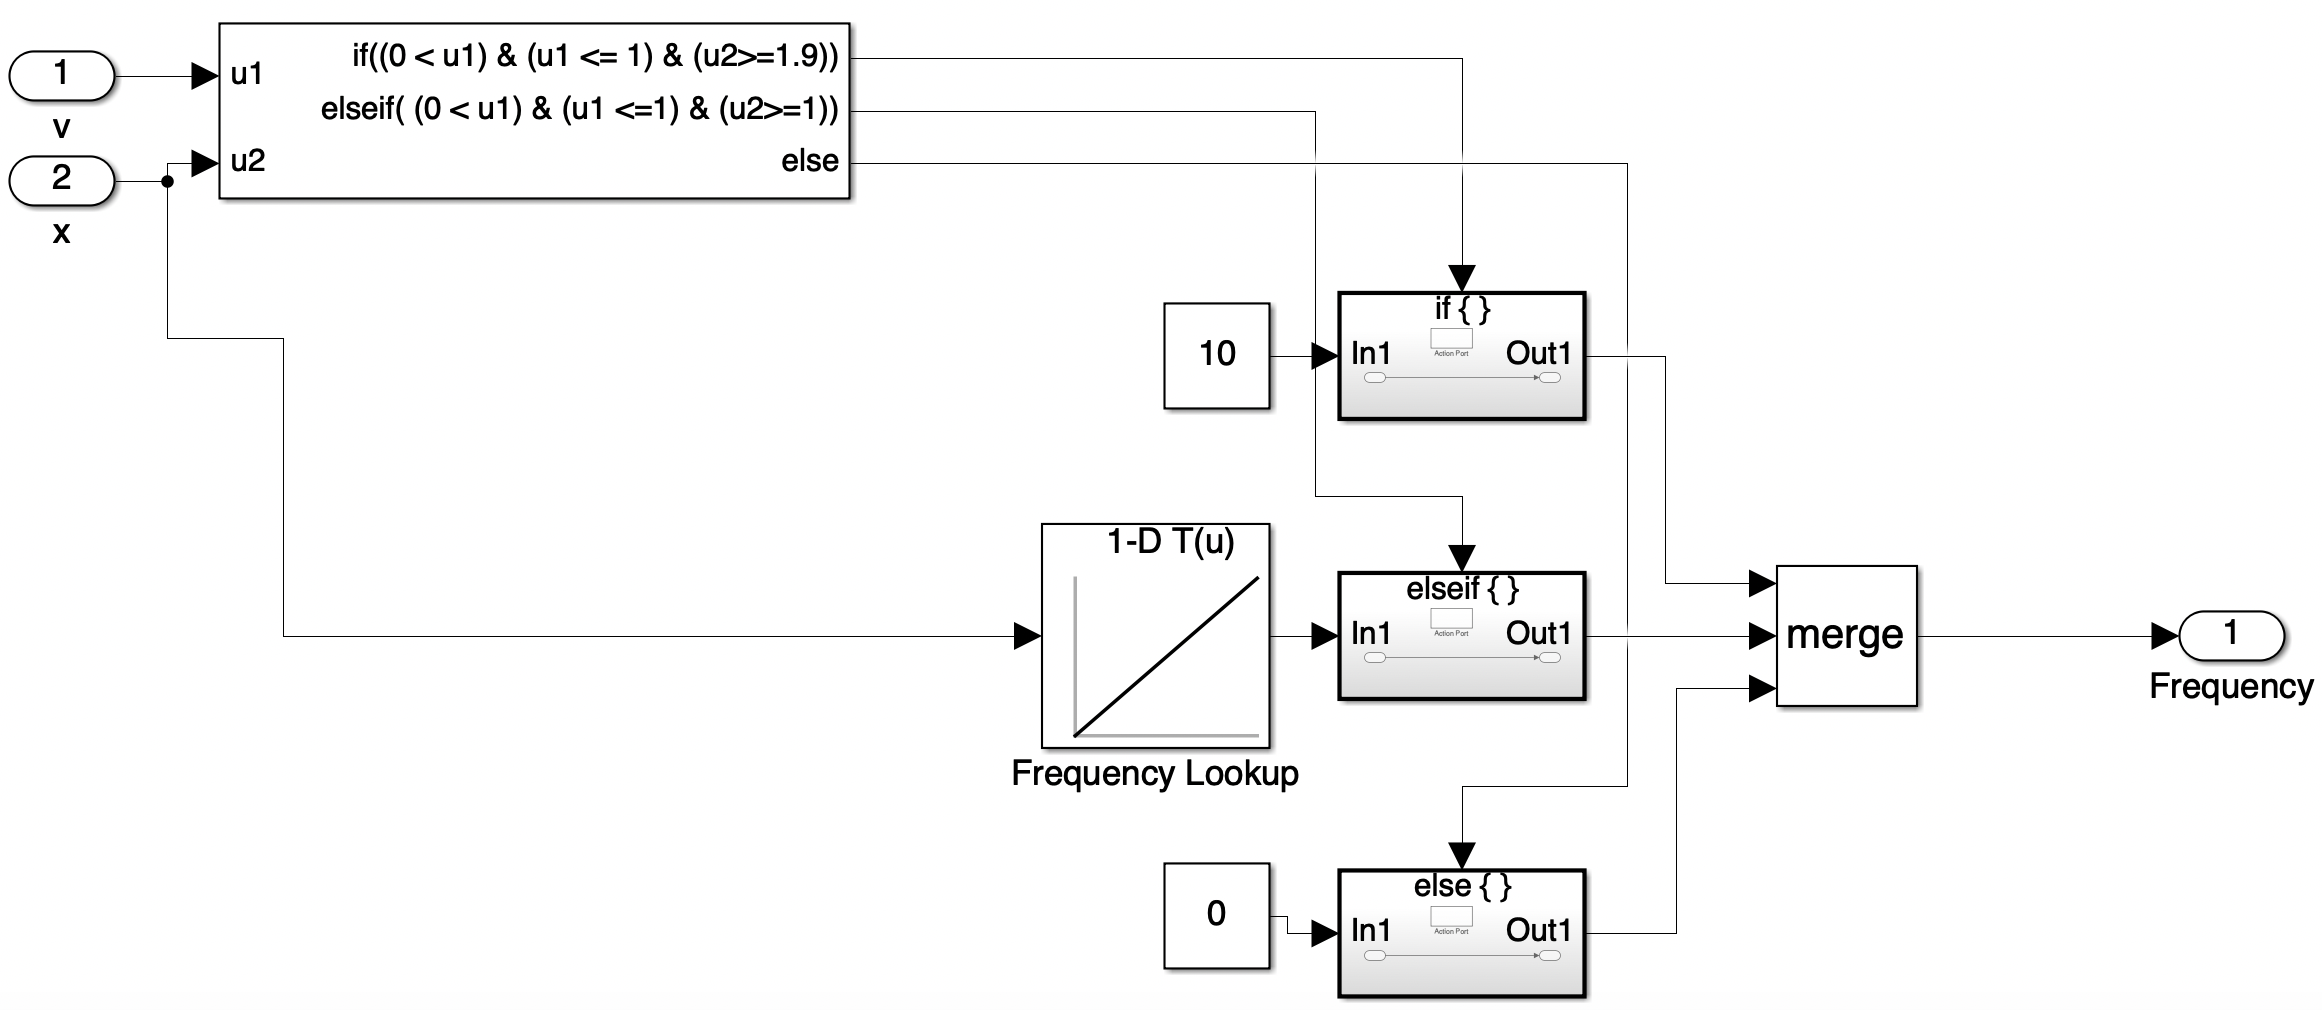
\includegraphics[width=1\textwidth]{images/D6_Frequency_Computation.png}
\caption{Simulink model of the frequency computation subsystem}
\label{fig:D6_Frequency_Computation}
\end{figure}

todo output plot
\section{Pulse signal generation}\label{sec:D6Signal}
Figure \ref{fig:D6_Pulse_Signal} shows the simulink model of the pulse signal generator.
This component provides a pulse signal with a variable frequency input.
The input is the output of the before described component.
Therefore if the input is 10, a continuous signal should be output.
This is realised by the if-condition, which, if the input signal is 10 provides a continuous high output.\\
If the frequency is 0, 0 should be output.\\
If that is not the case either the pulse signal is generated.
The frequency is the input to the integrator.
The integrator has a reset input port and will be reset after each period.
For each period the output of integrator will start at 0 and will go up to 1.
Until the output reaches 0.5 a high pulse will be output (50 \% duty cycle).
This is the purpose of the less or equal 0.5 check.
If the output of the integrator is greater that 0.5 a low pulse is output.

\begin{figure}[H]
\centering
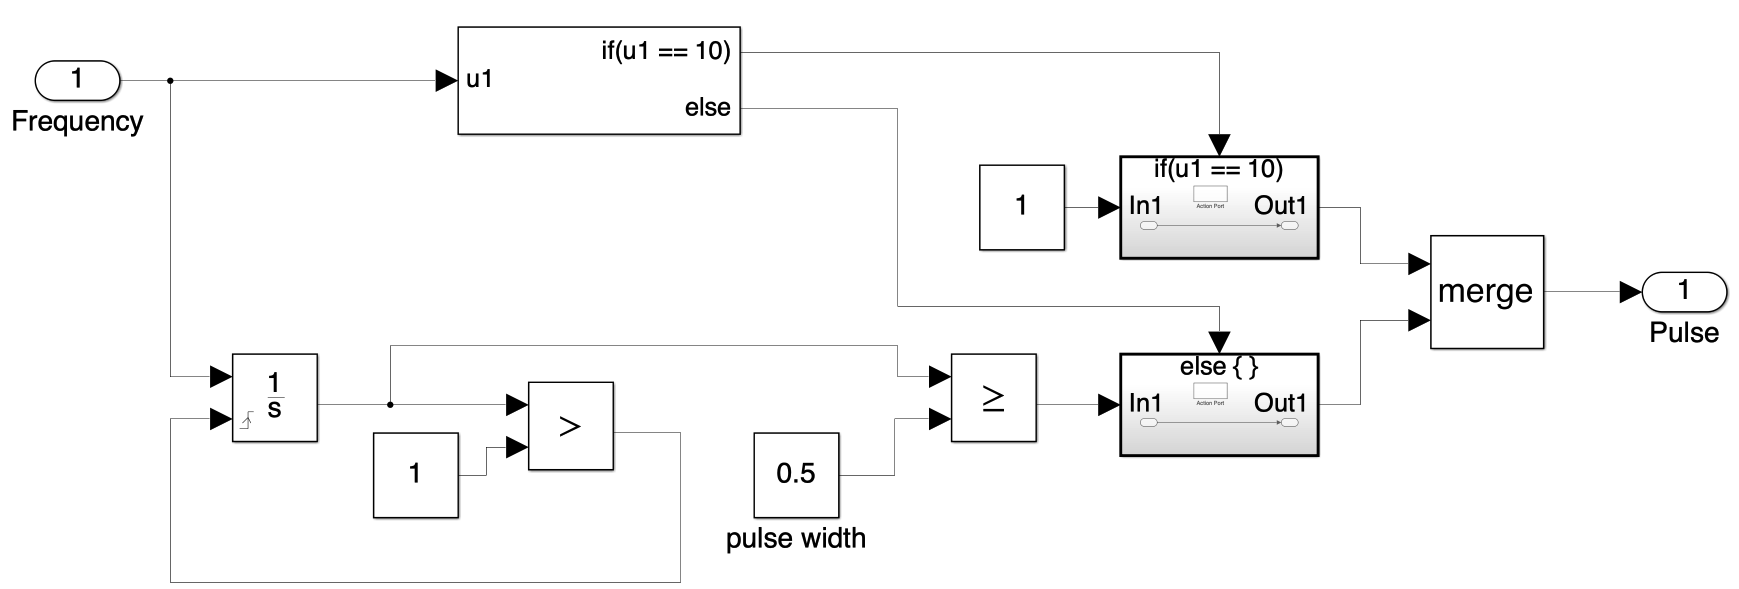
\includegraphics[width=1\textwidth]{images/D6_provide_signal.png}
\caption{Simulink model of the pulse generation subsystem}
\label{fig:D6_Pulse_Signal}
\end{figure}

\section{Integration into car model}\label{sec:D6Frequency}
Using subsystems for the developed components makes it easy to include into and extend the existing model, which can be seen in figure \ref{fig:D6_Integation}.
\begin{figure}[H]
\centering
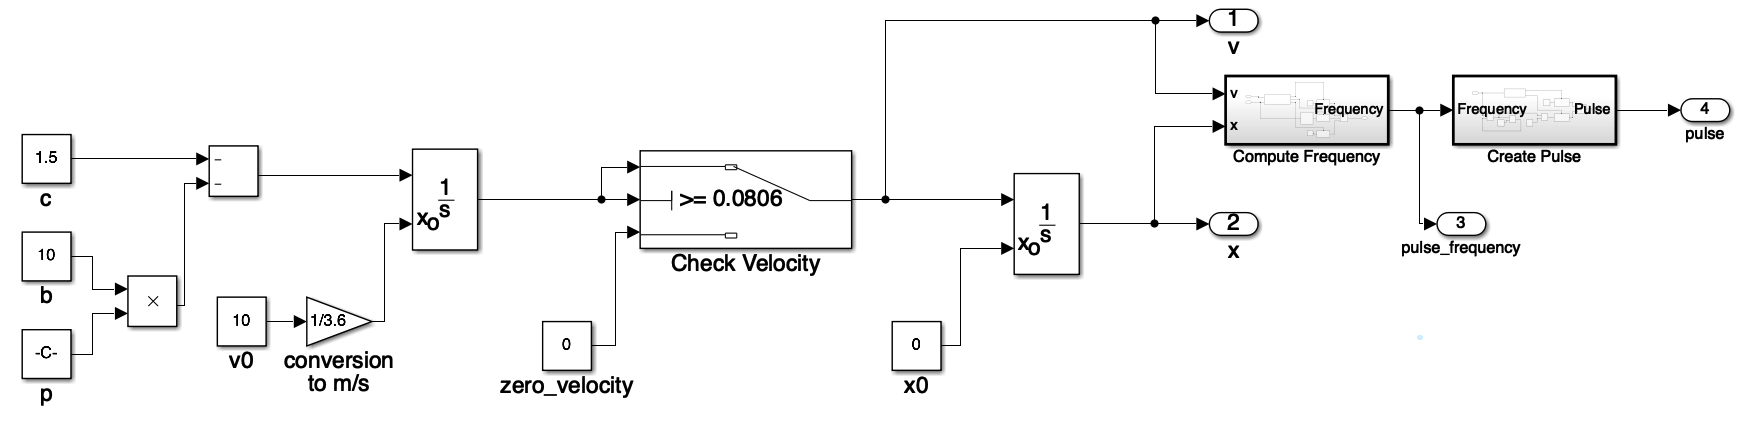
\includegraphics[width=1\textwidth]{images/D6_integration.png}
\caption{Simulink model of the car including the pulse signal}
\label{fig:D6_Integation}
\end{figure}

\section{Signal demonstration}\label{sec:D6_SignalDemonstration}

todo neu
\begin{figure}[H]
\centering
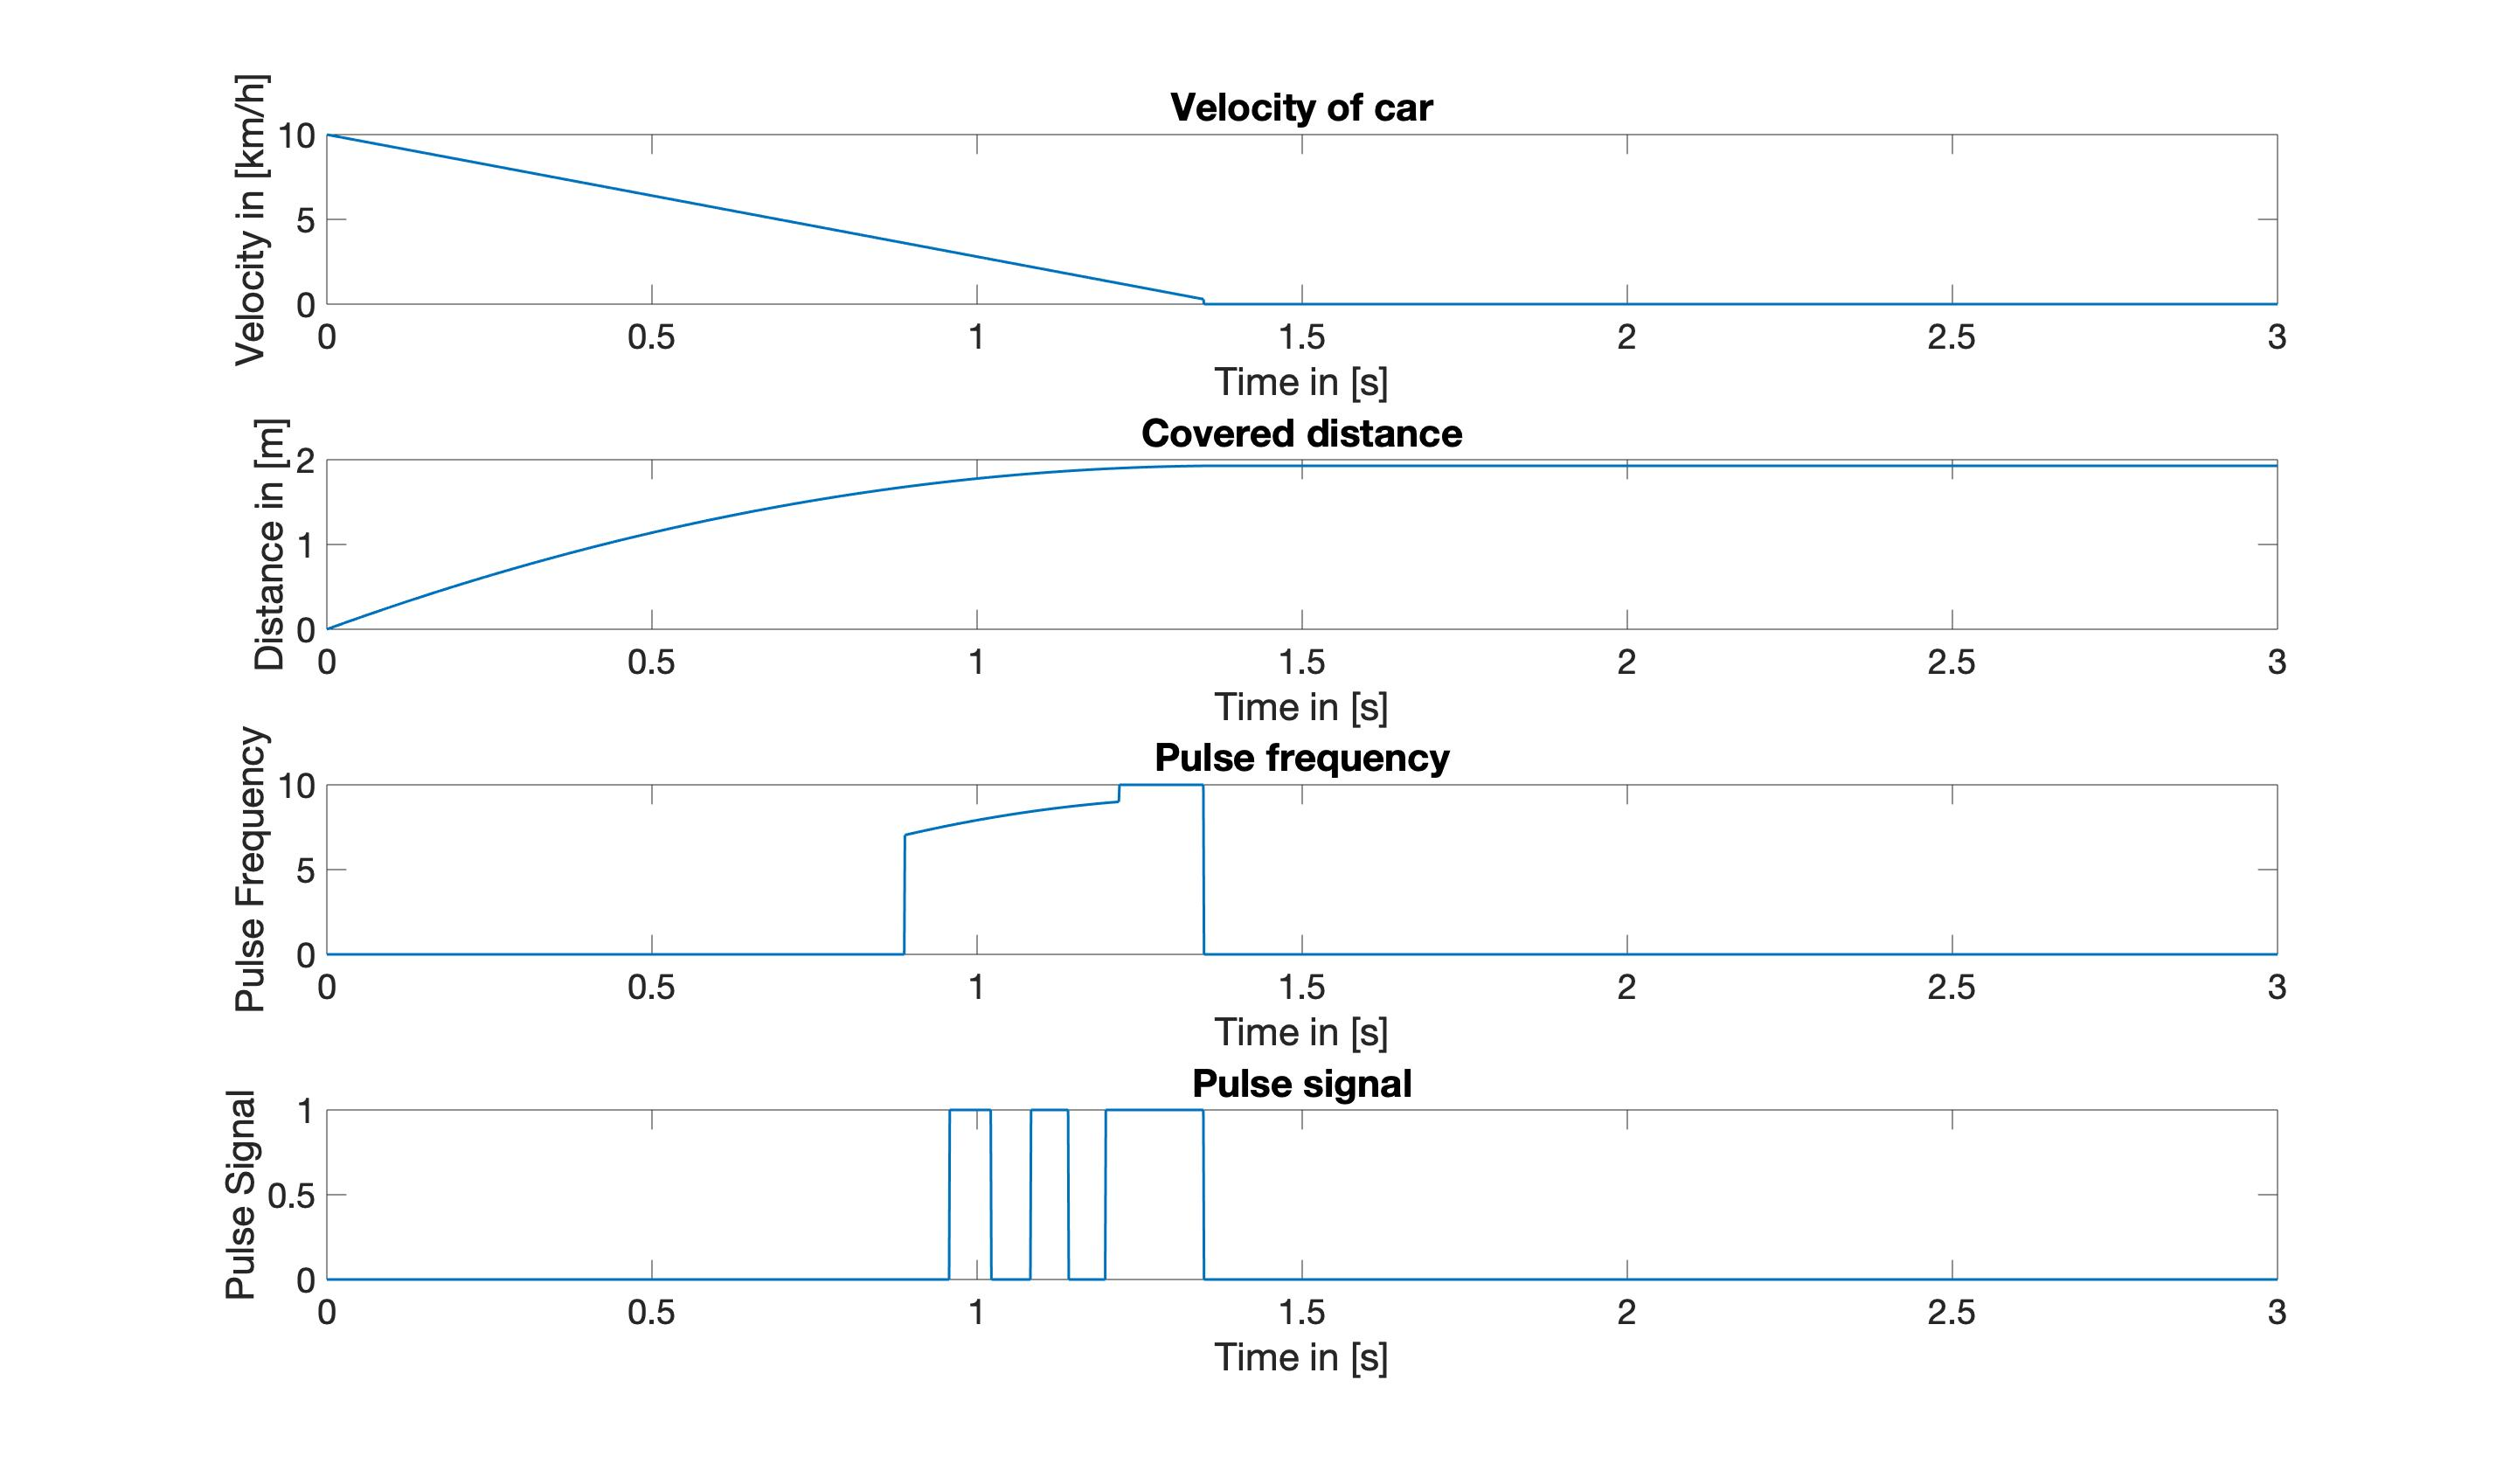
\includegraphics[width=1\textwidth]{images/D6_result.jpg}
\caption{Demonstration of pulse signal}
\label{fig:D6_Result}
\end{figure}

\chapter{D7: Transfer of Simulink model to ASCET}\label{cha:D7}
- integration block as combination of multiplication and addition

\begin{figure}[H]
\centering
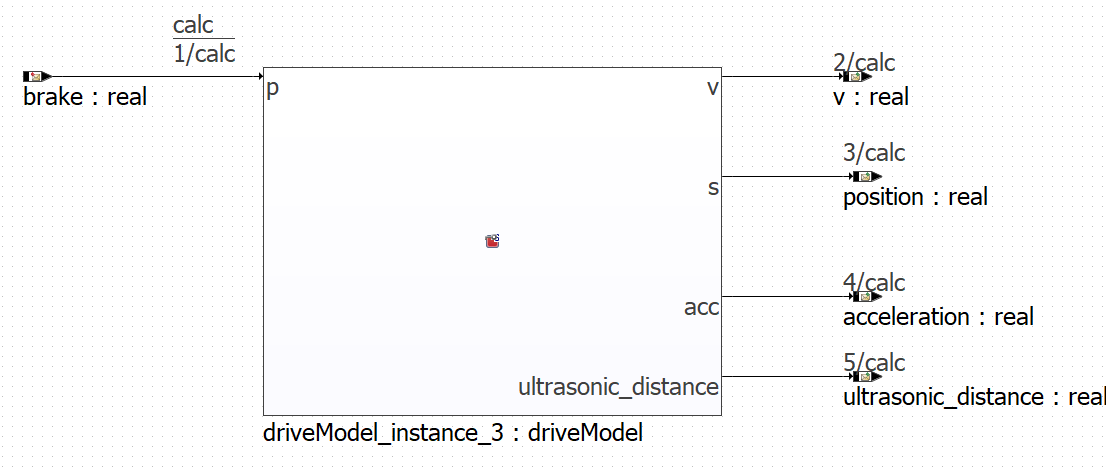
\includegraphics[width=1\textwidth]{images/Blockdiagramm_car.png}
\caption{ASCET Blockdiagramm of car}
\label{fig:BlockdiagrammCar}
\end{figure}

\begin{figure}[H]
\centering
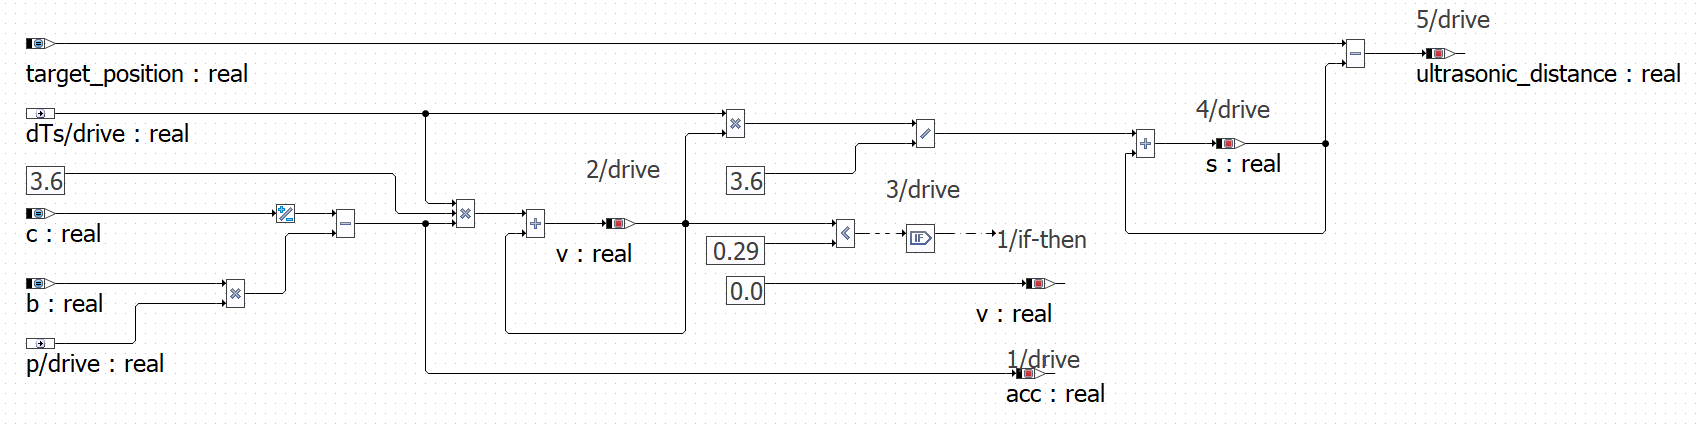
\includegraphics[width=1\textwidth]{images/Blockdiagramm_drivingmodel.png}
\caption{ASCET Blockdiagramm of driving model}
\label{fig:BlockdiagrammDrivingModel}
\end{figure}

\begin{figure}[H]
\centering
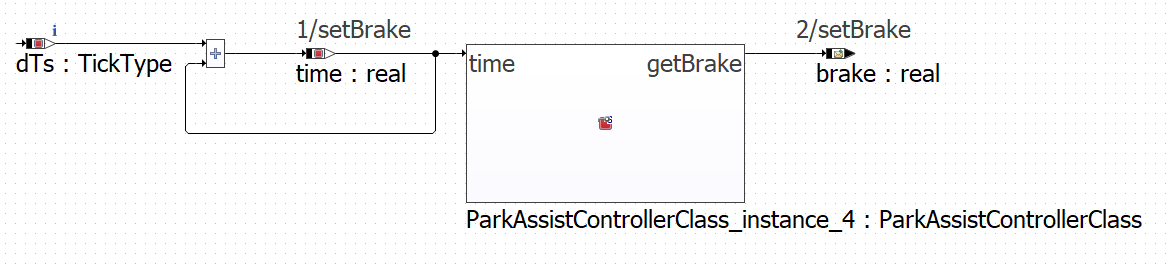
\includegraphics[width=1\textwidth]{images/Blockdiagramm_ParkAssistController.png}
\caption{ASCET Blockdiagramm of park assist controller}
\label{fig:BlockdiagrammParkAssistController}
\end{figure}

\begin{figure}[H]
\centering
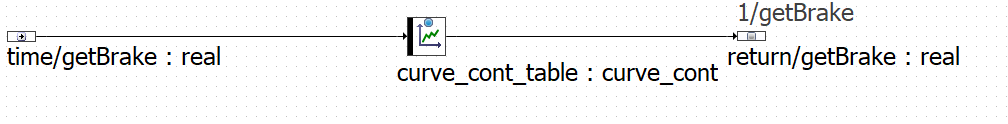
\includegraphics[width=1\textwidth]{images/Blockdiagramm_ParkAssistControllerClass.png}
\caption{ASCET Blockdiagramm of park assist controller class}
\label{fig:BlockdiagrammParkAssistControllerClass}
\end{figure}

\chapter{D8: Implementation of pulse signal in ASCET}\label{cha:D8}

- consists of two classes, one class calculates frequency, second class generates pulse signal \\
- frequency computation class connects two classes, passes calculated frequency to generate pulse signal \\
- input: velocity and position, dTs \\
- output: intern output: frequency, pulse signal \\

\begin{figure}[H]
\centering
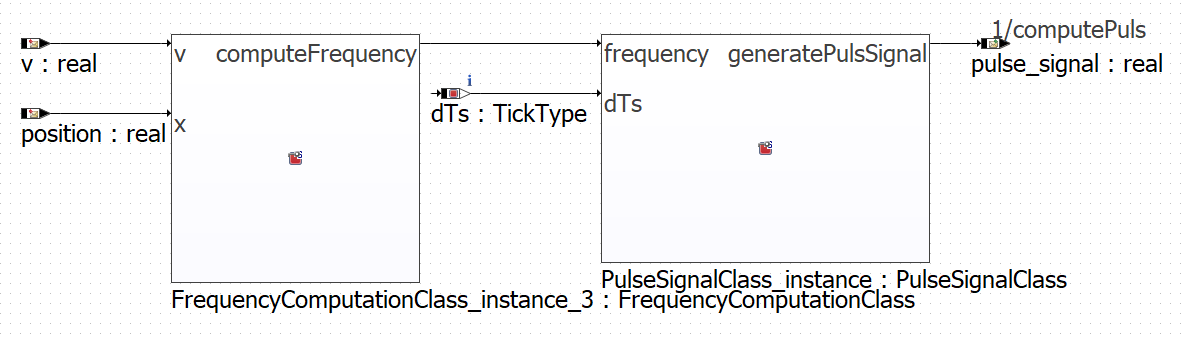
\includegraphics[width=1\textwidth]{images/Blockdiagramm_FrequencyComputation.png}
\caption{ASCET Blockdiagramm of frequency computation}
\label{fig:BlockdiagrammFrequencyComputation}
\end{figure}

- important: sequenzing \\
- input: velocity and position, if velocity greater zero and less or equal than 1 and if position greater than 1.9 meters return 10 for continuous pulse, else: check if position greater than 1, then frequency lookup table, else: return zero \\
\begin{figure}[H]
\centering
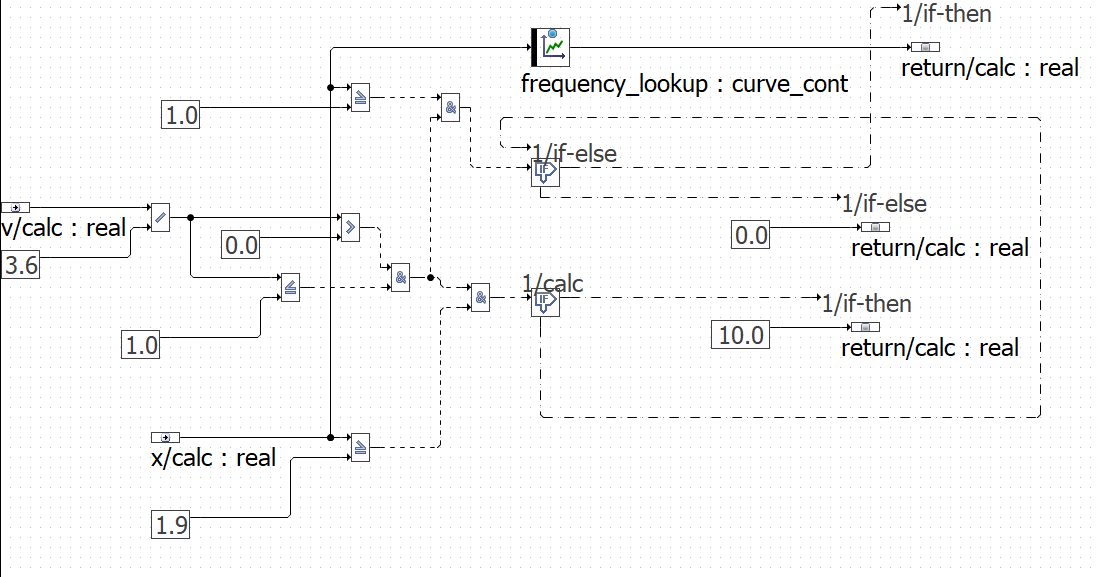
\includegraphics[width=1\textwidth]{images/Blockdiagramm_FrequencyComputationClass.png}
\caption{ASCET Blockdiagramm of frequency computation class}
\label{fig:BlockdiagrammFrequencyComputationClass}
\end{figure}

- if frequency zero, return 1, else: if frequency 0 return 0, else: integrate frequency, if integrated frequency greater than 0.5 (pulse width changes by changing this parameter, now half of period) return 1 else 0 so half of period signal high, other half low, reset integration if integrated frequency greater than 1 beziehungsweise if periode is over\\

\begin{figure}[H]
\centering
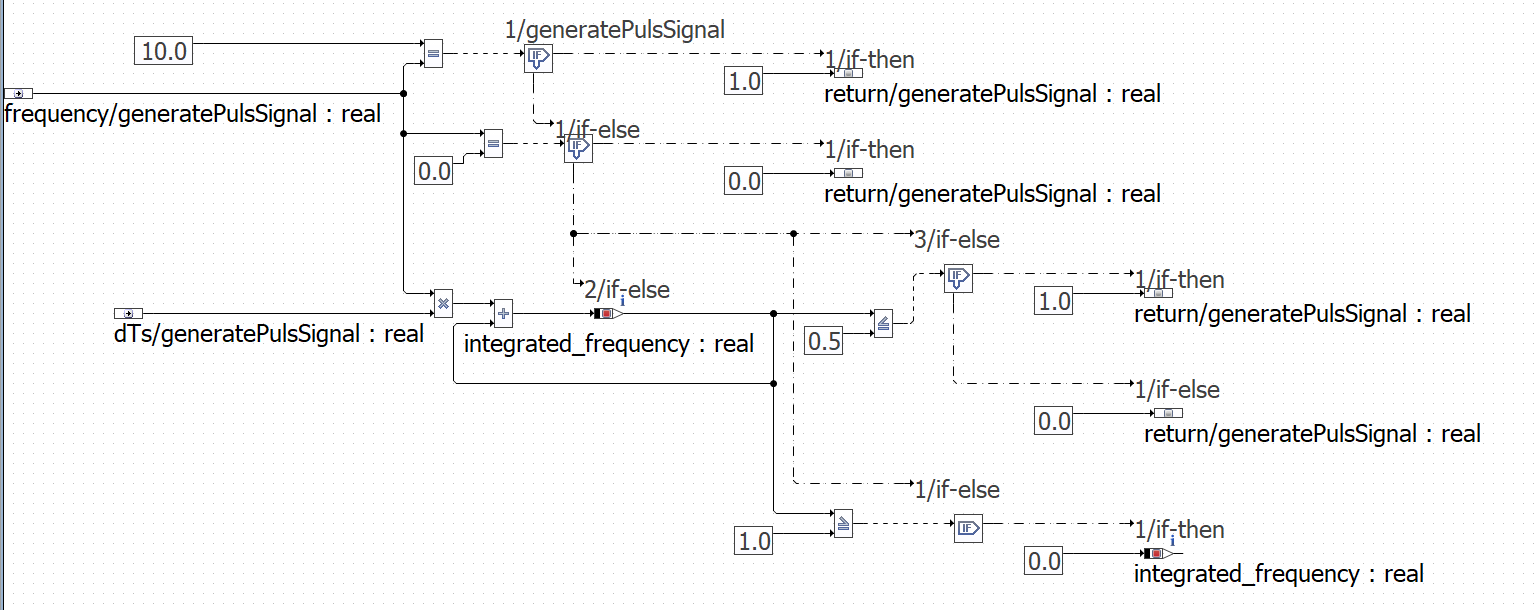
\includegraphics[width=1\textwidth]{images/Blockdiagramm_PulseSignalClass.png}
\caption{ASCET Blockdiagramm of pulse signal class}
\label{fig:BlockdiagrammPulseSignal}
\end{figure}



\chapter{D9: Implementation of unit tests for ASCET model parts}\label{cha:D9}
This section covers the unit tests of all components of the ASCET model.
The components were designed in a modular way to allow easy unit testing.
Also wrapper classes, passing messages into the components, are used to make it possible to unit test the components.
This is the only functionality the wrapper classes include.
That is necessary to make sure that no new bugs are introduced by the wrapper classes, because they can not be unit tested.\\
The unit tests are bundled in a package called $test$ in the ASCET project. The assertLib is imported for the assertions that are used in the unit tests. The unit tests are grouped by component with a static test class for each component. One test case corresponds to one method within the unit test classes.\\

Test cases are derived by analysing the requirements and finding equivalence classes.
The goal of the test case coverage is to cover equivalence class and in addition to that select values that might result in errors based on experience.s

- pulse signal, drive model not possible to unit test because of time component
- Messages erklären\\

\section{Unit tests for ParkAssistControl}

\section{Unit tests for pulse signal frequency generation}

\begin{table}[H]
\centering
\caption{Equivalence classes for unit testing pulse signal frequency generation}
\begin{adjustbox}{width=1\textwidth, center=\textwidth}
\renewcommand{\arraystretch}{1}
\begin{tabular}{lllllll}
\textbf{Position} & \textbf{Velocity} & \textbf{Output} \\\hline
irrelevant & v = 0m/s or v > 1m/s & Zero\\
1 m <= s <= 1.9 m  & 0 m/s < v <= 1 m/s & $f(s)=-7.889\; Hz + 8.889*s\; Hz$\\
1.9 m < s <= 2 m  & 0 m/s < v <= 1 m/s & Continuous (10)
\end{tabular}
\end{adjustbox}
\end{table}

Table \ref{tbl:D9_FrequencyGenerationTestCases} shows the test cases derived from the equivalence classes above.
\begin{table}[H]
\centering
\caption{Unit test test cases pulse signal frequency generation}
\begin{adjustbox}{width=1\textwidth, center=\textwidth}
\renewcommand{\arraystretch}{1}
\begin{tabular}{llll}
\textbf{Test case name}               & \textbf{Velocity {[}m/s{]}} & \textbf{Position {[}m{]}} & \textbf{Expected frequency} \\ \hline
continuousPulse                       & 0.5                         & 1.91                      & 10                                    \\
noFrequencyBecauseVelocityHigh        & 1.5                         & 1                         & 1                                     \\
noFrequencyBecauseVelocityZero        & 0                           & 1.8                       & 0                                     \\
noFrequencyBecausPosition             & 0.9                         & 0.9                       & 0                                     \\
noFrequencyBecauseVelocityAndPosition & 1.1                         & 0.9                       & 0                                     \\
frequencyLow                          & 1.0                         & 1.0                       & 1                                     \\
frequencyHigh                         & 1.0                         & 1.9                       & 9                                     \\
frequencyMid                          & 1.0                         & 1.5                       & 5.44 < result \textless 5.45 
\end{tabular}
\end{adjustbox}
\label{tbl:D9_FrequencyGenerationTestCases}
\end{table}

\section{Unit tests for pulse signal}
The table below shows the equivalence classes for the pulse signal.
\begin{table}[H]
\centering
\caption{Equivalence classes for unit testing pulse signal}
\begin{adjustbox}{width=1\textwidth, center=\textwidth}
\renewcommand{\arraystretch}{1}
\begin{tabular}{lllllll}
\textbf{Position} & \textbf{Velocity} & \textbf{Pulse Signal} \\\hline
irrelevant & V = 0m/s oder V > 1m/s & Zero\\
1m <= X <= 1.9m  & 0m/s < V <= 1m/s & Alternating 0,1\\
1.9m < X <= 2m  & 0m/s < V <= 1m/s &Continuous
\end{tabular}
\end{adjustbox}
\end{table}

-test cases

\begin{table}[H]
\centering
\caption{Pulse signal test cases}
\renewcommand{\arraystretch}{1}
\begin{tabular}{lll}
\textbf{Frequency} & \textbf{dts} & \textbf{Expected result} \\\hline
0         & 1   & 0               \\
10        & 1   & 1              
\end{tabular}
\end{table}


- Alternating pulse signal not possible to test because dependant of time 

\chapter{D10: Development and implementation of a system test environment for ASCET simulation}\label{cha:D10}

- wait 5 seconds until starting because ascet experiment environment does not display the first seconds \\
- in first 5 seconds brake = -0.15 to counter c and b, v = 0 \\
- after five seconds set v to 10 km/h and start experiment

\begin{figure}[H]
\centering
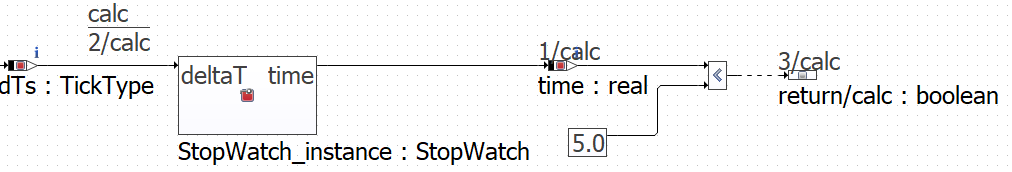
\includegraphics[width=1\textwidth]{images/Blockdiagramm_settings.png}
\caption{ASCET Blockdiagramm of settings}
\label{fig:BlockdiagrammSettings}
\end{figure}

\begin{figure}[H]
\centering
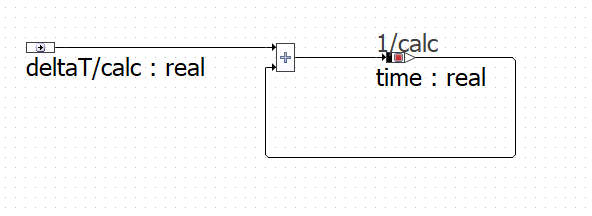
\includegraphics[width=1\textwidth]{images/Blockdiagramm_stopwatch.png}
\caption{ASCET Blockdiagramm of stopwatch}
\label{fig:BlockdiagrammStopwatch}
\end{figure}



\chapter{D11*: Plausibility check comparing measured velocities and distances}\label{cha:D11}
-statistically independent ultrasonic distance and velocity
-if distance to next object for ultrasonic sensor is known

-al
\chapter{D13*: Impact of inaccuracies}\label{cha:D13}
-ultrasonic measurement: what if object is round?
-
\chapter{D14*: Reflection}\label{cha:D14}
-only 2 meter stop considered
-model not realistic